%%%%%%%%%%%%%%%%%%%%%%%%%%%%% Thesis.tex %%%%%%%%%%%%%%%%%%%%%%%%%%%%%%%
%                                                                      %
%  ---------- Master of Science Dissertation template ----------       %
%                                                                      %
%  Template for the Master Thesis according to the regulations         %
%  published by the Academic Board (Direcção Académica) at IST.        %
%                                                                      %
%  For up-to-date guide, please refer to the official website          %
%
% https://tecnico.ulisboa.pt/pt/ensino/estudar-no-tecnico/informacoes-academicas/dissertacao-de-mestrado/
%                                                                      %
%       Andre C. Marta                                                 %
%       Area Cientifica de Mecanica Aplicada e Aeroespacial            %
%       Departamento de Engenharia Mecanica                            %
%       Instituto Superior Tecnico                                     %
%       Av. Rovisco Pais                                               %
%       1049-001 Lisboa                                                %
%       Portugal                                                       %
%       Tel: +351 21 841 9469                                          %
%                        3469 (extension)                              %
%       Email: andre.marta@tecnico.ulisboa.pt                          %
%                                                                      %
%  Created:       Jan 20, 2011                                         %
%  Last Modified: Mar  4, 2024                                         %
%                                                                      %
%%%%%%%%%%%%%%%%%%%%%%%%%%%%%%%%%%%%%%%%%%%%%%%%%%%%%%%%%%%%%%%%%%%%%%%%
%  Revision history                                                    %
%  v1 - 2011/01/24 - original template                                 %
%  v2 - 2012/10/30 - new IST image and glossary support                %
%  v3 - 2013/12/10 - update according to 2012/13 official guide        %
%  v4 - 2014/02/28 - new default for bibliography style                %
%  v5 - 2014/05/07 - update according to 2013/14 official guide        %
%  v6 - 2015/07/02 - cover page format fixed,                          %
%                    contents page numbering fixed,                    %
%                    better language support,                          %
%                    enhanced examples of tables,                      %
%                    new option for appendix page numbering format,    %
%                    custom bibliography style                         %
%  v7 - 2018/02/19 - multiple citations compressed                     %
%  v8 - 2019/05/13 - added examples (pseudo-code)                      %
%  v9 - 2020/03/03 - added French language support                     %
%                    indented first paragraphs                         %
%  v10- 2021/01/29 - place caption above table                         %
%  v11- 2022/06/29 - included Declaration of original work             %
%  v12- 2024/02/26 - new glossaries and subfig packages                %
%%%%%%%%%%%%%%%%%%%%%%%%%%%%%%%%%%%%%%%%%%%%%%%%%%%%%%%%%%%%%%%%%%%%%%%%
%                                                                      %
% To generate the PDF file, type "make" at the terminal prompt.        %
%                                                                      %
% This IST template LaTeX package was created by the author            %
% and it can be downloaded from:                                       %
%    https://fenix.tecnico.ulisboa.pt/homepage/ist31052/               %
% or https://mdo.tecnico.ulisboa.pt/templates/                         %
%                                                                      %
% The external packages can be downloaded from                         %
% the Comprehensive TeX Archive Network at http://www.ctan.org/        %
%                                                                      %
% List of LaTex symbols:                                               %
% http://www.ctan.org/tex-archive/info/symbols/comprehensive/          %
%                                                                      %
% Help with LaTex can be found at                                      %
% http://en.wikibooks.org/wiki/LaTeX                                   %
%%%%%%%%%%%%%%%%%%%%%%%%%%%%%%%%%%%%%%%%%%%%%%%%%%%%%%%%%%%%%%%%%%%%%%%%

%%%%%%%%%%%%%%%%%%%%%%%%%%%%%%%%%%%%%%%%%%%%%%%%%%%%%%%%%%%%%%%%%%%%%%%%
%     Preamble                                                         %
%%%%%%%%%%%%%%%%%%%%%%%%%%%%%%%%%%%%%%%%%%%%%%%%%%%%%%%%%%%%%%%%%%%%%%%%

% ----------------------------------------------------------------------
%  Set the document class
% ----------------------------------------------------------------------
\documentclass[10pt,a4paper,twoside]{report}

% ----------------------------------------------------------------------
% Define external packages, language, margins, fonts and new commands
% ----------------------------------------------------------------------
%%%%%%%%%%%%%%%%%%%%%%%%%%%%%%%%%%%%%%%%%%%%%%%%%%%%%%%%%%%%%%%%%%%%%%%%
%                                                                      %
%     File: Thesis_Preamble.tex                                        %
%     Tex Master: Thesis.tex                                           %
%                                                                      %
%     Author: Andre C. Marta                                           %
%     Last modified :  4 Mar 2024                                      %
%                                                                      %
%%%%%%%%%%%%%%%%%%%%%%%%%%%%%%%%%%%%%%%%%%%%%%%%%%%%%%%%%%%%%%%%%%%%%%%%

% 'natbib' package
%
% Flexible bibliography support.
% https://www.ctan.org/pkg/natbib
%
% > produce author-year style citations
%
% \citet  and \citep  for textual and parenthetical citations, respectively
% \citet* and \citep* that print the full author list, and not just the abbreviated one
% \citealt is the same as \citet but without parentheses. Similarly, \citealp is \citep without parentheses
% \citeauthor
% \citeyear
% \citeyearpar
%
%% natbib options can be provided when package is loaded \usepackage[options]{natbib}
%%
%% Following options are valid:
%%
%%   round  -  round parentheses are used (default)
%%   square -  square brackets are used   [option]
%%   curly  -  curly braces are used      {option}
%%   angle  -  angle brackets are used    <option>
%%   semicolon  -  multiple citations separated by semi-colon (default)
%%   colon  - same as semicolon, an earlier confusion
%%   comma  -  separated by comma
%%   authoryear - for author–year citations (default)
%%   numbers-  selects numerical citations
%%   super  -  numerical citations as superscripts, as in Nature
%%   sort   -  sorts multiple citations according to order in ref. list
%%   sort&compress   -  like sort, but also compresses numerical citations
%%   compress - compresses without sorting
%%
% ******************************* SELECT *******************************
%\usepackage{natbib}          % <<<<< References in alphabetical list Correia, Silva, ...
\usepackage[numbers,sort&compress]{natbib} % <<<<< References in numbered list [1],[2],...
% ******************************* SELECT *******************************


% 'notoccite' package
%
% Prevent trouble from citations in table of contents, etc.
% http://ctan.org/pkg/notoccite
%
% > If you have \cite commands in \section-like commands, or in \caption,
%   the citation will also appear in the table of contents, or list of whatever.
%   If you are also using an unsrt-like bibliography style, these citations will
%   come at the very start of the bibliography, which is confusing. This pack­age
%   suppresses the effect.
%
\usepackage{notoccite}


% ----------------------------------------------------------------------
% Define document language.
% ----------------------------------------------------------------------

% 'inputenc' package
%
% Accept different input encodings.
% https://www.ctan.org/pkg/inputenc
%
% > allows typing non-english text in LaTeX sources.
%
% ******************************* SELECT *******************************
%\usepackage[latin1]{inputenc} % <<<<< Windows
\usepackage[utf8]{inputenc}   % <<<<< Linux
% ******************************* SELECT *******************************

% 'babel' package
%
% Multilingual support for Plain TeX or LaTeX.
% https://www.ctan.org/pkg/babel
%
% > sets the variable names according to the language selected
%
% ******************************* SELECT *******************************
%\usepackage[portuguese]{babel} % <<<<< Portuguese
\usepackage[english]{babel} % <<<<< English
%\usepackage[francais]{babel} % <<<<< French (requires package texlive-lang-french)
% ******************************* SELECT *******************************

% 'nomencl' package
%
% Produce lists of symbols as in nomenclature.
% https://www.ctan.org/pkg/nomencl
%
% The nomencl package makes use of the MakeIndex program
% in order to produce the nomenclature list.
%
% Nomenclature
% 1) On running the file through LATEX, the command \makenomenclature
%    in the preamble instructs it to create/open the nomenclature file
%    <jobname>.nlo corresponding to the LATEX file <jobname>.tex and
%    writes the information from the \nomenclature commands to this file.
% 2) The next step is to invoke MakeIndex in order to produce the
%    <jobname>.nls file. This can be achieved by making use of the
%    command: makeindex <jobname>.nlo -s nomencl.ist -o <jobname>.nls
% 3) The last step is to invoke LATEX on the <jobname>.tex file once
%    more. There, the \printnomenclature in the document will input the
%    <jobname>.nls file and process it according to the given options.
%
% Nomenclature (produces *.nlo *.nls files)
\usepackage{nomencl}
\makenomenclature
%
% Group variables according to their symbol type
% (see <prefix> in Thesis_Nomenclature.tex)
%
\RequirePackage{ifthen} 
\ifthenelse{\equal{\languagename}{english}}%
    { % English
    \renewcommand{\nomgroup}[1]{%
      \ifthenelse{\equal{#1}{R}}{%
        \item[\textbf{Roman symbols}]}{%
        \ifthenelse{\equal{#1}{G}}{%
          \item[\textbf{Greek symbols}]}{%
          \ifthenelse{\equal{#1}{S}}{%
            \item[\textbf{Subscripts}]}{%
            \ifthenelse{\equal{#1}{T}}{%
              \item[\textbf{Superscripts}]}{}}}}}%
    }{%
    \ifthenelse{\equal{\languagename}{french}}%
    { % French
    \renewcommand{\nomgroup}[1]{%
      \ifthenelse{\equal{#1}{R}}{%
        \item[\textbf{Symbole romains}]}{%
        \ifthenelse{\equal{#1}{G}}{%
          \item[\textbf{Symboles grecs}]}{%
          \ifthenelse{\equal{#1}{S}}{%
            \item[\textbf{Indices}]}{% lettre inférieure
            \ifthenelse{\equal{#1}{T}}{%
              \item[\textbf{Exposants}]}{}}}}}% lettre supérieure
    }{ % Portuguese
    \renewcommand{\nomgroup}[1]{%
      \ifthenelse{\equal{#1}{R}}{%
        \item[\textbf{Simbolos romanos}]}{%
        \ifthenelse{\equal{#1}{G}}{%
          \item[\textbf{Simbolos gregos}]}{%
          \ifthenelse{\equal{#1}{S}}{%
            \item[\textbf{Subscritos}]}{%
            \ifthenelse{\equal{#1}{T}}{%
              \item[\textbf{Sobrescritos}]}{}}}}}%
    }}%


% 'glossaries' package
%
% Create glossaries and lists of acronyms
% https://www.ctan.org/pkg/glossaries
%
% The glossaries package makes use of the MakeIndex program
% in order to produce the glossary list.
%
% The following options are used:
%   - acronym      : to produce the list of acronyms
%   - nonumberlist : to remove the page number
%   - nopostdot    : to remove the dot at the end of definition of term
%   - nogroupskip  : to remove the line spacing between groups
%
% Glossary (produces *.glo *.ist files)
%
\usepackage[acronym,nonumberlist,nopostdot,nogroupskip]{glossaries}
\setglossarystyle{long}
\renewcommand{\glsnamefont}[1]{\textbf{#1}} % acronym in bold face
%\makeglossaries


% List of LaTeX variable names: \abstractname, \appendixname, \bibname,
%   \chaptername, \contentsname, \listfigurename, \listtablename, ...)
% https://texfaq.org/FAQ-fixnam
%
% Changing the words babel uses (uncomment and redefine as necessary...)
%
\newcommand{\acknowledgments}{@undefined} % new LaTeX variable name
%
% > English
%
\addto\captionsenglish{\renewcommand{\acknowledgments}{Acknowledgments}}
%\addto\captionsenglish{\renewcommand{\contentsname}{Contents}}
%\addto\captionsenglish{\renewcommand{\listtablename}{List of Tables}}
%\addto\captionsenglish{\renewcommand{\listfigurename}{List of Figures}}
%\addto\captionsenglish{\renewcommand{\nomname}{Nomenclature}} % (List of Symbols)
%\addto\captionsenglish{\renewcommand{\glossaryname}{Glossary}}
\addto\captionsenglish{\renewcommand{\acronymname}{Glossary}} % Acronyms
%\addto\captionsenglish{\renewcommand{\bibname}{References}} % Bibliography
%\addto\captionsenglish{\renewcommand{\appendixname}{Appendix}}

% > French
%
\addto\captionsfrench{\renewcommand{\acknowledgments}{Remerciements}}
%\addto\captionsfrench{\renewcommand{\contentsname}{Table des matières}}
%\addto\captionsfrench{\renewcommand{\listtablename}{Liste des tableaux}}
\addto\captionsfrench{\renewcommand{\listfigurename}{Liste des figures}} % Table des figures
%\addto\captionsfrench{\renewcommand{\nomname}{Nomenclature}}
%\addto\captionsfrench{\renewcommand{\glossaryname}{Glossaire}}
%\addto\captionsfrench{\renewcommand{\acronymname}{Liste des acronymes}}
%\addto\captionsfrench{\renewcommand{\bibname}{Bibliographie}}
%\addto\captionsfrench{\renewcommand{\appendixname}{Annexe}}

% > Portuguese
%
\addto\captionsportuguese{\renewcommand{\acknowledgments}{Agradecimentos}}
%\addto\captionsportuguese{\renewcommand{\contentsname}{Conte\'{u}do}}
%\addto\captionsportuguese{\renewcommand{\listtablename}{Lista de Figuras}}
%\addto\captionsportuguese{\renewcommand{\listfigurename}{Lista de Tabelas}}
\addto\captionsportuguese{\renewcommand{\nomname}{Lista de S\'{i}mbolos}} % Nomenclatura
%\addto\captionsportuguese{\renewcommand{\glossaryname}{Gloss\'{a}rio}}
%\addto\captionsportuguese{\renewcommand{\acronymname}{Lista de Abrevia\c{c}\~{o}es}}
%\addto\captionsportuguese{\renewcommand{\bibname}{Refer\^{e}ncias}} % Bibliografia
%\addto\captionsportuguese{\renewcommand{\appendixname}{Anexo}} % Apendice


% ----------------------------------------------------------------------
% Define cover fields in both english and portuguese.
% ----------------------------------------------------------------------
%
\newcommand{\coverThesis}{@undefined} % new LaTeX variable name
\newcommand{\coverSupervisors}{@undefined} % new LaTeX variable name
\newcommand{\coverExaminationCommittee}{@undefined} % new LaTeX variable name
\newcommand{\coverChairperson}{@undefined} % new LaTeX variable name
\newcommand{\coverSupervisor}{@undefined} % new LaTeX variable name
\newcommand{\coverMemberCommittee}{@undefined} % new LaTeX variable name
% > English
\addto\captionsenglish{\renewcommand{\coverThesis}{Thesis to obtain the Master of Science Degree in}}
\addto\captionsenglish{\renewcommand{\coverSupervisors}{Supervisor(s)}}
\addto\captionsenglish{\renewcommand{\coverExaminationCommittee}{Examination Committee}}
\addto\captionsenglish{\renewcommand{\coverChairperson}{Chairperson}}
\addto\captionsenglish{\renewcommand{\coverSupervisor}{Supervisor}}
\addto\captionsenglish{\renewcommand{\coverMemberCommittee}{Member of the Committee}}
% > French
\addto\captionsfrench{\renewcommand{\coverThesis}{Th\`ese pour l'obtention du Maîtrise des Sciences en}}
\addto\captionsfrench{\renewcommand{\coverSupervisors}{Directeur(s) de th\`ese}}
\addto\captionsfrench{\renewcommand{\coverExaminationCommittee}{Jury}}
\addto\captionsfrench{\renewcommand{\coverChairperson}{Pr\'esident}}
\addto\captionsfrench{\renewcommand{\coverSupervisor}{Directeur de th\`ese}}
\addto\captionsfrench{\renewcommand{\coverMemberCommittee}{Rapporteur}}
% > Portuguese
\addto\captionsportuguese{\renewcommand{\coverThesis}{Disserta\c{c}\~{a}o para obten\c{c}\~{a}o do Grau de Mestre em}}
\addto\captionsportuguese{\renewcommand{\coverSupervisors}{Orientador(es)}}
\addto\captionsportuguese{\renewcommand{\coverExaminationCommittee}{J\'{u}ri}}
\addto\captionsportuguese{\renewcommand{\coverChairperson}{Presidente}}
\addto\captionsportuguese{\renewcommand{\coverSupervisor}{Orientador}}
\addto\captionsportuguese{\renewcommand{\coverMemberCommittee}{Vogal}}


% ----------------------------------------------------------------------
% Define Declaration of original work in both english and portuguese.
% ----------------------------------------------------------------------
%
\newcommand{\declarationTitle}{@undefined} % new LaTeX variable name
\newcommand{\declarationText}{@undefined}  % new LaTeX variable name
% > English
\addto\captionsenglish{\renewcommand{\declarationTitle}{Declaration}}
\addto\captionsenglish{\renewcommand{\declarationText}{I declare that this document is an original work of my own authorship and that it fulfills all the requirements of the Code of Conduct and Good Practices of the Universidade de Lisboa.}}
% > Portuguese
\addto\captionsportuguese{\renewcommand{\declarationTitle}{Declara\c{c}\~{a}o}}
\addto\captionsportuguese{\renewcommand{\declarationText}{Declaro que o presente documento \'{e} um trabalho original da minha autoria e que cumpre todos os requisitos do C\'{o}digo de Conduta e Boas Pr\'{a}ticas da Universidade de Lisboa.}}


% ----------------------------------------------------------------------
% Define default and cover page fonts.
% ----------------------------------------------------------------------

% Use Arial font as default
%
\renewcommand{\rmdefault}{phv}
\renewcommand{\sfdefault}{phv}

% Define cover page fonts
%
%         encoding     family       series      shape
%  \usefont{T1}     {phv}=helvetica  {b}=bold    {n}=normal
%                   {ptm}=times      {m}=normal  {sl}=slanted
%                                                {it}=italic
% see more examples at
% https://www.overleaf.com/learn/latex/Font_typefaces
% https://tug.org/FontCatalogue/
%
\def\FontLn{% 16 pt normal
  \usefont{T1}{phv}{m}{n}\fontsize{16pt}{16pt}\selectfont}
\def\FontLb{% 16 pt bold
  \usefont{T1}{phv}{b}{n}\fontsize{16pt}{16pt}\selectfont}
\def\FontMn{% 14 pt normal
  \usefont{T1}{phv}{m}{n}\fontsize{14pt}{14pt}\selectfont}
\def\FontMb{% 14 pt bold
  \usefont{T1}{phv}{b}{n}\fontsize{14pt}{14pt}\selectfont}
\def\FontSn{% 12 pt normal
  \usefont{T1}{phv}{m}{n}\fontsize{12pt}{12pt}\selectfont}


% ----------------------------------------------------------------------
% Define page margins and line spacing.
% ----------------------------------------------------------------------

% 'geometry' package
%
% Flexible and complete interface to document dimensions.
% https://www.ctan.org/pkg/geometry
%
% > set the page margins (2.5cm minimum in every side, as per IST rules)
%
\usepackage{geometry}	
\geometry{a4paper,
         tmargin=2.5cm, bmargin=2.5cm,
         lmargin=2.5cm, rmargin=2.5cm,
         verbose=false}

% 'setspace' package
%
% Set space between lines.
% https://www.ctan.org/pkg/setspace
%
% > allow setting line spacing (line spacing of 1.5, as per IST rules)
%
\usepackage{setspace}
\renewcommand{\baselinestretch}{1.5}


% ----------------------------------------------------------------------
% Define paragraph formating.
% ----------------------------------------------------------------------

% 'indentfirst' package
%
% Indent first paragraph after section header.
% https://ctan.org/pkg/indentfirst
%
% > indent all paragraphs (as per IST rules)
%
\usepackage{indentfirst}	


% ----------------------------------------------------------------------
% Include other external packages.
% Note that not all of these packages may be available on all system
% installations. If necessary, include the .sty files locally in
% the Thesis.tex file directory.
% ----------------------------------------------------------------------

% 'graphicx' package
%
% Enhanced support for graphics.
% https://www.ctan.org/pkg/graphicx
%
% > extends arguments of the \includegraphics command
%
\usepackage{graphicx}


% 'amsmath' package
%
% AMS mathematical facilities for LaTeX.
% https://www.ctan.org/pkg/amsmath
%
% > American Mathematical Society (AMS) plain Tex macros
%
\usepackage{amsmath}  % AMS mathematical facilities for LaTeX.
\usepackage{amsthm}   % Typesetting theorems (AMS style).
\usepackage{amsfonts} % TeX fonts from the AMS


% 'subfig' package
%
% Figures broken into subfigures.
% https://www.ctan.org/pkg/subfig
%
% > support for the manipulation and reference of subfigures
%
\usepackage{subfig}


% 'ar' package
%
% Capital A and capital R ligature for Aspect Ratio.
% https://www.ctan.org/pkg/aspectratio
%
% > provides the "aspect ratio" symbol with command \AR
%
\usepackage{ar}


% 'url' package
%
% Verbatim with URL-sensitive line breaks.
% https://www.ctan.org/pkg/url
%
% > URLs in BibTex
%
% \usepackage{url}


% 'varioref' package
%
% Intelligent page references.
% https://www.ctan.org/pkg/varioref
%
% > smart page, figure, table and equation referencing
%
%\usepackage{varioref}


% 'dcolumn' package
%
% Align on the decimal point of numbers in tabular columns.
% https://www.ctan.org/pkg/dcolumn
%
% > decimal-aligned tabular math columns
%
\usepackage{dcolumn}
\newcolumntype{d}{D{.}{.}{-1}} % column aligned by the point separator '.'
\newcolumntype{e}{D{E}{E}{-1}} % column aligned by the exponent 'E'


% 'verbatim' package
%
% Reimplementation of and extensions to LaTeX verbatim.
% https://www.ctan.org/pkg/verbatim
%
% > provides the verbatim environment (\begin{verbatim},\end{verbatim})
%   and a comment environment (\begin{comment},  \end{comment})
%
% \usepackage{verbatim}


% 'moreverb' package
%
% Extended verbatim.
% https://www.ctan.org/pkg/moreverb
%
% > supports tab expansion and line numbering
%
% \usepackage{moreverb}


% 'rotating' package
%
% Rotation tools, including rotated full-page floats.
% https://www.ctan.org/pkg/rotating
%
% > show wide figures and tables in landscape format:
%   use \begin{sidewaystable} and \begin{sidewaysfigure}
%   instead of 'table' and 'figure', respectively.
%
\usepackage{rotating}


% 'hyperref' package
%
% Extensive support for hypertext in LaTeX.
% https://www.ctan.org/pkg/hyperref
%
% > Extends the functionality of all the LATEX cross-referencing
%   commands (including the table of contents, bibliographies etc) to
%   produce \special commands which a driver can turn into hypertext
%   links; Also provides new commands to allow the user to write adhoc
%   hypertext links, including those to external documents and URLs.
%
\usepackage[pdftex]{hyperref} % enhance documents that are to be
                              % output as HTML and PDF
\hypersetup{colorlinks,       % color text of links and anchors,
                              % eliminates borders around links
%            linkcolor=red,    % color for normal internal links
            linkcolor=black,  % color for normal internal links
            anchorcolor=black,% color for anchor text
%            citecolor=green,  % color for bibliographical citations
            citecolor=black,  % color for bibliographical citations
%            filecolor=magenta,% color for URLs which open local files
            filecolor=black,  % color for URLs which open local files
%            menucolor=red,    % color for Acrobat menu items
            menucolor=black,  % color for Acrobat menu items
%            urlcolor=cyan,    % color for linked URLs
            urlcolor=black,   % color for linked URLs
	          bookmarks=true,         % create PDF bookmarks
	          bookmarksopen=false,    % don't expand bookmarks
	          bookmarksnumbered=true, % number bookmarks
	          pdftitle={Thesis},
            pdfauthor={Andre C. Marta},
            pdfsubject={Thesis Title},
            pdfkeywords={Thesis Keywords},
            pdfstartview=FitV,
            pdfdisplaydoctitle=true}


% 'hypcap' package
%
% Adjusting the anchors of captions.
% https://www.ctan.org/pkg/hypcap
%
% > fixes the problem with hyperref, that links to floats points
%   below the caption and not at the beginning of the float.
%
\usepackage[figure,table]{hypcap}


% 'multirow' package
%
% Create tabular cells spanning multiple rows
% http://www.ctan.org/pkg/multirow
%
\usepackage{multirow}


% 'booktabs' package
%
% Publication quality tables in LaTeX
% http://www.ctan.org/pkg/booktabs
%
% > enhance the quality of tables in LaTeX, providing extra commands.
%
% \renewcommand{\arraystretch}{<ratio>} % space between rows
%
\usepackage{booktabs}
%\newcommand{\ra}[1]{\renewcommand{\arraystretch}{#1}}


% 'pdfpages' package
%
% Include PDF documents in LaTeX
% http://www.ctan.org/pkg/pdfpages
%
% > inclusion of external multi-page PDF documents in LaTeX documents.
%   Pages may be freely selected and similar to psnup it is possible to put
%   several logical pages onto each sheet of paper.
%
% \includepdf{filename.pdf}
% \includepdf[pages={4-9},nup=2x3,landscape=true]{filename.pdf}
%
\usepackage{pdfpages}


% 'algorithmicx' package
%
% The algorithmic style you always wanted
% https://ctan.org/pkg/algorithmicx
%
% > provides many possibilities to customizethe layout of algorithms.  You can use one of the predefined layouts(pseudocode,pascalandcand others), with or without modifications,or you can define a completely new layout for your specific needs
%
\usepackage{algorithm}
\usepackage{algpseudocode}


% ----------------------------------------------------------------------
% Define new commands to assure consistent treatment throughout document
% ----------------------------------------------------------------------

\newcommand{\ud}{\mathrm{d}}                % total derivative
\newcommand{\degree}{\ensuremath{^\circ\,}} % degrees

% Abbreviations

\newcommand{\mcol}{\multicolumn}            % table format

\newcommand{\eqnref}[1]{(\ref{#1})}
\newcommand{\class}[1]{\texttt{#1}}
\newcommand{\package}[1]{\texttt{#1}}
\newcommand{\file}[1]{\texttt{#1}}
\newcommand{\BibTeX}{\textsc{Bib}\TeX}

% Typefaces ( example: {\bf Bold text here} )
%
% > pre-defined
%   \bf % bold face
%   \it % italic
%   \tt % typewriter
%
% > newly defined
\newcommand{\tr}[1]{{\ensuremath{\textrm{#1}}}}   % text roman
\newcommand{\tb}[1]{{\ensuremath{\textbf{#1}}}}   % text bold face
\newcommand{\ti}[1]{{\ensuremath{\textit{#1}}}}   % text italic
\newcommand{\mc}[1]{{\ensuremath{\mathcal{#1}}}}  % math calygraphy
\newcommand{\mco}[1]{{\ensuremath{\mathcalold{#1}}}}% math old calygraphy
\newcommand{\mr}[1]{{\ensuremath{\mathrm{#1}}}}   % math roman
\newcommand{\mb}[1]{{\ensuremath{\mathbf{#1}}}}   % math bold face
\newcommand{\bs}[1]{\ensuremath{\boldsymbol{#1}}} % math symbol
\def\bm#1{\mathchoice                             % math bold
  {\mbox{\boldmath$\displaystyle#1$}}%
  {\mbox{\boldmath$#1$}}%
  {\mbox{\boldmath$\scriptstyle#1$}}%
  {\mbox{\boldmath$\scriptscriptstyle#1$}}}
\newcommand{\boldcal}[1]{{\ensuremath{\boldsymbol{\mathcal{#1}}}}}% math bold calygraphy
 % file "Thesis_Preamble.tex"

% ----------------------------------------------------------------------
% Entries of nomenclature and glossary
% included before \begin{document} to avoid paging misbehaviours
% ----------------------------------------------------------------------

% entries of nomenclature (list of symbols)
%%%%%%%%%%%%%%%%%%%%%%%%%%%%%%%%%%%%%%%%%%%%%%%%%%%%%%%%%%%%%%%%%%%%%%%%
%                                                                      %
%     File: Thesis_Nomenclature.tex                                    %
%     Tex Master: Thesis.tex                                           %
%                                                                      %
%     Author: Andre C. Marta                                           %
%     Last modified : 27 Feb 2024                                      %
%                                                                      %
%%%%%%%%%%%%%%%%%%%%%%%%%%%%%%%%%%%%%%%%%%%%%%%%%%%%%%%%%%%%%%%%%%%%%%%%
%
% The definitions can be placed anywhere in the document body
% and their order is sorted by <symbol> automatically when
% calling makeindex in the makefile
%
% The \glossary command has the following syntax:
%
% \glossary{entry}
%
% The \nomenclature command has the following syntax:
%
% \nomenclature[<prefix>]{<symbol>}{<description>}
%
% where <prefix> is used for fine tuning the sort order,
% <symbol> is the symbol to be described, and <description> is
% the actual description.
% The first letter in <prefix> indicates the group, while the next
% (if included) help sorting if the <symbol> is not a plain character
%
% ----------------------------------------------------------------------
% Roman symbols [r]
%\nomenclature[ru]{$\bf u$}{Velocity vector}
%\nomenclature[ru]{$u,v,w$}{Velocity Cartesian components}
%\nomenclature[rp]{$p$}{Pressure}
%\nomenclature[rC]{$C_D$}{Coefficient of drag}
%\nomenclature[rC]{$C_L$}{Coefficient of lift}
%\nomenclature[rC]{$C_M$}{Coefficient of moment}

% ----------------------------------------------------------------------
% Greek symbols [g]
%\nomenclature[g]{$\rho$}{Density}
%\nomenclature[g]{$\alpha$}{Angle of attack}
%\nomenclature[g]{$\beta$}{Angle of side-slip}
%\nomenclature[g]{$\mu$}{Molecular viscosity coefficient}
%\nomenclature[g]{$\kappa$}{Thermal conductivity coefficient}

% ----------------------------------------------------------------------
% Subscripts [s]
%\nomenclature[sx]{$x,y,z$}{Cartesian components}
%\nomenclature[si]{$i,j,k$}{Computational indexes}
%\nomenclature[s]{$\infty$}{Free-stream condition}
%\nomenclature[sr]{ref}{Reference condition}
%\nomenclature[sn]{$n$}{Normal component}

% ----------------------------------------------------------------------
% Supercripts [t]
%\nomenclature[t]{T}{Transpose}
%\nomenclature[t]{*}{Adjoint}
 % file "Thesis_Nomenclature.tex"

% entries of glossary (list of acronyms)
%%%%%%%%%%%%%%%%%%%%%%%%%%%%%%%%%%%%%%%%%%%%%%%%%%%%%%%%%%%%%%%%%%%%%%%%
%                                                                      %
%     File: Thesis_Glossary.tex                                        %
%     Tex Master: Thesis.tex                                           %
%                                                                      %
%     Author: Andre C. Marta                                           %
%     Last modified : 27 Feb 2024                                      %
%                                                                      %
%%%%%%%%%%%%%%%%%%%%%%%%%%%%%%%%%%%%%%%%%%%%%%%%%%%%%%%%%%%%%%%%%%%%%%%%
%
% The definitions can be placed anywhere in the document body
% and their order is sorted by <key> automatically when
% calling makeindex in the makefile
%
% ----------------------------------------------------------------------
% To create a glossary entry, use the following syntax:
%
% \newglossaryentry{<label>}{name={<key>}, description={<value>}}
%
% where the parameters are:
% <label> is the label of the entry,
% <key> is the acronym to be defined by the glossary entry (in lowercase, preferably)
% <value> is the actual definition of the current term
%
% To produce the desired term in the document, that will be replaced by
% the user-defined in the output, use the following syntax:
%
% \gls{<label>}
%
% ----------------------------------------------------------------------
% To create a acronym entry, use the following syntax:
%
% \newacronym{⟨label⟩}{⟨abbrv⟩}{⟨full⟩}
%
% where the parameters are:
% <label> is the label of the entry,
% <abbrv> is the acronym,
% <full> is the definition of the acronym
%
% To produce the desired term in the document, that will be replaced by
% the user-defined in the output, use one of the following syntaxes:
%
% \acrlong{<label>}
% \acrshort{<label>}
% \acrfull{<label>}
%
% ----------------------------------------------------------------------
% By default, only those entries defined in the main document using the
% commands above will be displayed in the glossary (list of acronyms),
% unless the command \glsaddall is used,
% ----------------------------------------------------------------------

% The order of the definitions below is irrelevant
% since the glossary is automatically ordered alphabetically

\newacronym{amr}{AMR}{Adaptive Mesh Refinement}
\newacronym{ghg}{GHG}{Generalized Harmonic Gauge}
\newacronym{ligo}{LIGO}{Laser Interferometer Gravitational-Wave Observatory}
\newacronym{pde}{PDE}{Partial Differential Equation}


%\newacronym{⟨label⟩}{⟨abbrv⟩}{⟨full⟩}
%\newacronym{⟨label⟩}{⟨abbrv⟩}{⟨full⟩}
%\newacronym{⟨label⟩}{⟨abbrv⟩}{⟨full⟩}

% ----------------------------------------------------------------------
% displays all entries (even those unused with commands \acrlong/short/full)
\glsaddall

% ----------------------------------------------------------------------
% vertical aligment of acronyms' long names
\setlength\LTleft{0pt}
\setlength\LTright{0pt}
\setlength\glsdescwidth{1.0\hsize}
     % file "Thesis_Glossary.tex"


%%%%%%%%%%%%%%%%%%%%%%%%%%%%%%%%%%%%%%%%%%%%%%%%%%%%%%%%%%%%%%%%%%%%%%%%
%     Begin Document                                                   %
%%%%%%%%%%%%%%%%%%%%%%%%%%%%%%%%%%%%%%%%%%%%%%%%%%%%%%%%%%%%%%%%%%%%%%%%
\begin{document}

% Set plain page style (no headers, footer with centered page number)
\pagestyle{plain}

% Set roman numbering (i,ii,...) before the start of chapters
\pagenumbering{roman}

% ----------------------------------------------------------------------
%  Cover page
% ----------------------------------------------------------------------
%%%%%%%%%%%%%%%%%%%%%%%%%%%%%%%%%%%%%%%%%%%%%%%%%%%%%%%%%%%%%%%%%%%%%%%%
%                                                                      %
%     File: Thesis_FrontCover.tex                                      %
%     Tex Master: Thesis.tex                                           %
%                                                                      %
%     Author: Andre C. Marta                                           %
%     Last modified : 27 Feb 2024                                      %
%                                                                      %
%%%%%%%%%%%%%%%%%%%%%%%%%%%%%%%%%%%%%%%%%%%%%%%%%%%%%%%%%%%%%%%%%%%%%%%%

\thispagestyle {empty}

% IST Logo - Signature A
% parameters: bb=llx lly urx ury (bounding box), width=h_length, height=v_length, angle=angle, scale=factor, clip=true/false, draft=true/false. 

\includegraphics[bb=9.5cm 11cm 0cm 0cm,scale=0.29]{Figures/IST_A_CMYK_POS.pdf}

\begin{center}
%
% Figure (Image or plot)
\vspace{2.5cm}
% height = 50 mm
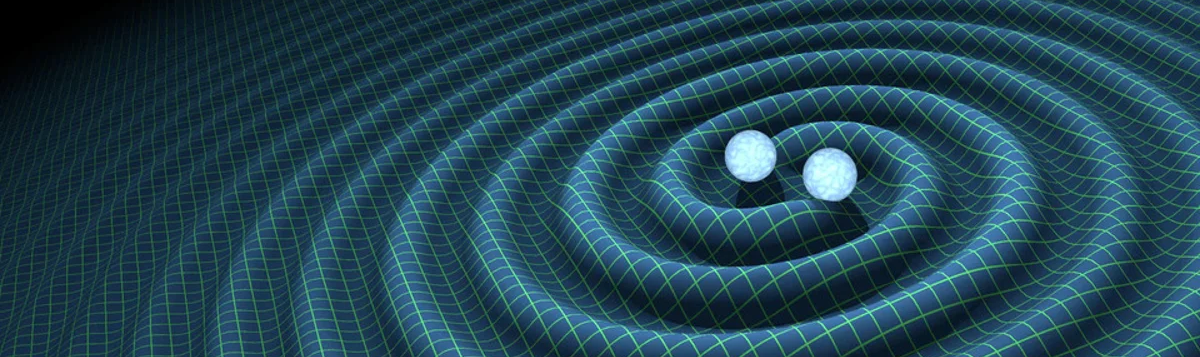
\includegraphics[width=\textwidth]{Figures/Cover_Image_cut.png} \\ % <<<<< EDIT FIGURE

% Title, author and degree
\vspace{1.0cm}
{\FontLb Linearized General Relativity in Hyperboloidal Coordinates} \\ % <<<<< EDIT TITLE
%\vspace{0.2cm}
%{\FontMn Subtitle (optional)} \\
%\vspace{1.9cm}
\vspace{2.6cm}
{\FontMb Filipe Ficalho} \\ % <<<<< EDIT NAME
\vspace{2.0cm}
{\FontSn \coverThesis} \\
\vspace{0.3cm}
{\FontLb Physics Engineering} \\ % <<<<< EDIT COURSE
\vspace{1.0cm}
{\FontSn %
\begin{tabular}{ll}
 \coverSupervisors: & Prof. David Hilditch
\end{tabular} } \\
\vspace{1.0cm}
{\FontMb \coverExaminationCommittee} \\
\vspace{0.3cm}
{\FontSn %
\begin{tabular}{c}
\coverChairperson:     Prof. Name 1  \\ % <<<<< EDIT NAME
\coverSupervisor:      Prof. David Hilditch  \\ % <<<<< EDIT NAME
\coverMemberCommittee: Prof. Name 2     % <<<<< EDIT NAME
\end{tabular} } \\
\vspace{1.5cm}
{\FontMb October 2025} \\ % <<<<< EDIT DATE (corresponds to date of oral examination)
%
\end{center}
 % file "Thesis_FrontCover.tex"
\cleardoublepage

% ----------------------------------------------------------------------
% Dedication page (optional)
% ----------------------------------------------------------------------
%%%%%%%%%%%%%%%%%%%%%%%%%%%%%%%%%%%%%%%%%%%%%%%%%%%%%%%%%%%%%%%%%%%%%%%%
%                                                                      %
%     File: Thesis_Dedication.tex                                      %
%     Tex Master: Thesis.tex                                           %
%                                                                      %
%     Author: Andre C. Marta                                           %
%     Last modified :  2 Jul 2015                                      %
%                                                                      %
%%%%%%%%%%%%%%%%%%%%%%%%%%%%%%%%%%%%%%%%%%%%%%%%%%%%%%%%%%%%%%%%%%%%%%%%

\null\vskip5cm%
\begin{flushright}
     Dedicated to someone special...
\end{flushright}
\vfill\newpage

 % file "Thesis_Dedication.tex"
\cleardoublepage

% ----------------------------------------------------------------------
% Declaration page (mandatory)
% ----------------------------------------------------------------------
%%%%%%%%%%%%%%%%%%%%%%%%%%%%%%%%%%%%%%%%%%%%%%%%%%%%%%%%%%%%%%%%%%%%%%%%
%                                                                      %
%     File: Thesis_Declaration.tex                                     %
%     Tex Master: Thesis.tex                                           %
%                                                                      %
%     Author: Andre C. Marta                                           %
%     Last modified :  29 Jun 2022                                     %
%                                                                      %
%%%%%%%%%%%%%%%%%%%%%%%%%%%%%%%%%%%%%%%%%%%%%%%%%%%%%%%%%%%%%%%%%%%%%%%%

\null\vskip5cm%
\begin{flushleft}
	\declarationTitle \\
	\declarationText
\end{flushleft}
\vfill\newpage

 % file "Thesis_Declaration.tex"
\cleardoublepage

% ----------------------------------------------------------------------
%  Acknowledgments (optional)
% ----------------------------------------------------------------------
%%%%%%%%%%%%%%%%%%%%%%%%%%%%%%%%%%%%%%%%%%%%%%%%%%%%%%%%%%%%%%%%%%%%%%%%
%                                                                      %
%     File: Thesis_Acknowledgments.tex                                 %
%     Tex Master: Thesis.tex                                           %
%                                                                      %
%     Author: Andre C. Marta                                           %
%     Last modified :  2 Jul 2015                                      %
%                                                                      %
%%%%%%%%%%%%%%%%%%%%%%%%%%%%%%%%%%%%%%%%%%%%%%%%%%%%%%%%%%%%%%%%%%%%%%%%

\section*{\acknowledgments}

% Add entry in the table of contents as section
\addcontentsline{toc}{section}{\acknowledgments}

A few words about the university, financial support, research advisor, dissertation readers, faculty or other professors, lab mates, other friends and family...

 % file "Thesis_Acknowledgements.tex"
\cleardoublepage

% ----------------------------------------------------------------------
%  Abstract (both in English and Portuguese)
% ----------------------------------------------------------------------
%%%%%%%%%%%%%%%%%%%%%%%%%%%%%%%%%%%%%%%%%%%%%%%%%%%%%%%%%%%%%%%%%%%%%%%%
%                                                                      %
%     File: Thesis_Resumo.tex                                          %
%     Tex Master: Thesis.tex                                           %
%                                                                      %
%     Author: Andre C. Marta                                           %
%     Last modified :  4 Mar 2024                                      %
%                                                                      %
%%%%%%%%%%%%%%%%%%%%%%%%%%%%%%%%%%%%%%%%%%%%%%%%%%%%%%%%%%%%%%%%%%%%%%%%

\section*{Resumo}

% Add entry in the table of contents as section
\addcontentsline{toc}{section}{Resumo}

Inserir o resumo em Portugu\^{e}s aqui com um máximo de 250 palavras e acompanhado de 4 a 6 palavras-chave.

\vfill

\textbf{\Large Palavras-chave:} palavra-chave1, palavra-chave2, palavra-chave3,...

   % file "Thesis_Resumo.tex"
\cleardoublepage

%%%%%%%%%%%%%%%%%%%%%%%%%%%%%%%%%%%%%%%%%%%%%%%%%%%%%%%%%%%%%%%%%%%%%%%%
%                                                                      %
%     File: Thesis_Abstract.tex                                        %
%     Tex Master: Thesis.tex                                           %
%                                                                      %
%     Author: Andre C. Marta                                           %
%     Last modified :  4 Mar 2024                                      %
%                                                                      %
%%%%%%%%%%%%%%%%%%%%%%%%%%%%%%%%%%%%%%%%%%%%%%%%%%%%%%%%%%%%%%%%%%%%%%%%

\section*{Abstract}

% Add entry in the table of contents as section
\addcontentsline{toc}{section}{Abstract}

Insert your abstract here with a maximum of 250 words, followed by 4 to 6 keywords.

\vfill

\textbf{\Large Keywords:} keyword1, keyword2, keyword3,...

 % file "Thesis_Abstract.tex"
\cleardoublepage

% ----------------------------------------------------------------------
%  Table of contents, list of tables, list of figures and nomenclature
% ----------------------------------------------------------------------

% Table of contents
%
\tableofcontents
\cleardoublepage 

% List of tables
%
% Add entry in the table of contents as section
\phantomsection
\addcontentsline{toc}{section}{\listtablename}
% Generate list
\listoftables
\cleardoublepage 

% List of figures
%
% Add entry in the table of contents as section
\phantomsection
\addcontentsline{toc}{section}{\listfigurename}
% Generate list
\listoffigures
\cleardoublepage 

% Nomenclature
%
% Add entry in the table of contents as section
\phantomsection
\addcontentsline{toc}{section}{\nomname}
% Insert nomenclature section produced by \makenomenclature
\printnomenclature
\cleardoublepage

% Glossary
%
% Add entry in the table of contents as section
\phantomsection
\addcontentsline{toc}{section}{\acronymname}
% Insert glossary section produced by \makeglossaries
\printglossary[type=\acronymtype,title=\acronymname, toctitle=\acronymname]
%\printglossary[type=\acronymtype,style=long,title=\acronymname, toctitle=\acronymname]
\cleardoublepage

% Set arabic numbering (1,2,...) after preface
%
\setcounter{page}{1}
\pagenumbering{arabic}

% ----------------------------------------------------------------------
%  Chapters
% ----------------------------------------------------------------------

%%%%%%%%%%%%%%%%%%%%%%%%%%%%%%%%%%%%%%%%%%%%%%%%%%%%%%%%%%%%%%%%%%%%%%%%
%                                                                      %
%     File: Thesis_Introduction.tex                                    %
%     Tex Master: Thesis.tex                                           %
%                                                                      %
%     Author: Andre C. Marta                                           %
%     Last modified :  4 Mar 2024                                      %
%                                                                      %
%%%%%%%%%%%%%%%%%%%%%%%%%%%%%%%%%%%%%%%%%%%%%%%%%%%%%%%%%%%%%%%%%%%%%%%%

\chapter{Introduction}
\label{chapter:introduction}


%%%%%%%%%%%%%%%%%%%%%%%%%%%%%%%%%%%%%%%%%%%%%%%%%%%%%%%%%%%%%%%%%%%%%%%%
\section{Motivation}
\label{section:motivation}

Gravitational waves have been in the minds of physicists since Albert Einstein first predicted their existence in 1916 as perturbations in the curvature of spacetime that propagate at the speed of light. However, it was not until nearly a century later, in 2015, that the \acrfull{ligo} made the first direct detection of this fascinating phenomenon \cite{PhysRevLett.116.061102}. This groundbreaking observation not only confirmed a key prediction of Einstein's general theory of relativity but also inaugurated the field of gravitational-wave astronomy, opening an entirely new window through which to observe and understand the universe.

Gravitational waves immediately caught the attention of the scientific community due to their unique interaction with matter. Unlike electromagnetic waves, which can be absorbed, scattered, or reprocessed by intervening media, gravitational waves propagate essentially unimpeded from their astrophysical sources to Earth. This property allows them to carry direct information about highly energetic and compact systems, including binary black hole mergers, neutron star collisions, and potentially processes in the early universe that are otherwise inaccessible to conventional astronomical methods.

Even though this new method of observation opens the door to a wealth of scientific opportunities, it also presents significant challenges. The signals detected by \acrshort{ligo} and other gravitational wave observatories are incredibly weak by the time they reach Earth, necessitating extremely sensitive detectors and sophisticated data analysis techniques to extract meaningful information from the noise. In order to interpret these signals accurately, it is crucial to have precise theoretical models of the gravitational waveforms produced by various astrophysical events. This is where numerical relativity comes into play, providing the tools to simulate the complex dynamics of spacetime and matter under extreme conditions. However, given the distance of Earth from the sources of gravitational waves, to predict the signals that detectors will observe, we must be able to extract the gravitational waves at null infinity, which is a significant challenge in itself. 

State-of-the-art numerical relativity codes, such as the Einstein Toolkit \cite{einstein_toolkit_2025}, do not have this capability built in, working around this issue by calculating the wave front at different radii and then extrapolating the results until future null infinity, which naturally comes at the cost of some amount of systematic error on the results. In this work, we present an alternative to the current methodology by evolving toy models for gravitational waves in a compactified spacetime, thereby bypassing the need for extrapolation.


%%%%%%%%%%%%%%%%%%%%%%%%%%%%%%%%%%%%%%%%%%%%%%%%%%%%%%%%%%%%%%%%%%%%%%%%
\section{Topic Overview}
\label{section:overview}

In a quest to upgrade the current state-of-the-art numerical relativity codes, which can only solve spherically symmetric models of General Relativity, to a full 3D code compatible with hyperboloidal layers, some work has been done. While some authors focus on the development of the mathematical tools required to evolve \acrfull{pde} systems on hyperboloidal layers \cite{hypmath1,hypmath2,hypmath3,hypmath4,Hyperboloidal_layers_for_hyperbolic_equations_on_unbounded_domains,Dual_Foliation_Formulations_of_General_Relativity}, others work on its implementation both in finite difference codes \cite{hypfinitediff1,hypfinitediff2,hypfinitediff3,hypfinitediff4,hypfinitediff5,hypfinitediff6,hypfinitediff7} and in spectral ones \cite{The_evolution_of_hyperboloidal_data_with_the_dual_foliation_formalism_Mathematical_analysis_and_wave_equation_tests} using different models for the creation and propagation of gravitational waves. Continuing this line of research, this thesis focuses on solving the wave equation and the cubic wave equation in hyperboloidal slices and hyperboloidal layers using spectral methods in full 3D with \acrfull{amr}. The wave equation serves as a toy model for gravitational waves, allowing us to test and validate our numerical methods in a simpler context before tackling the more complex equations of General Relativity. 

The cubic wave equation, on the other hand, introduces non-linearities that are more representative of the challenges faced in simulating realistic astrophysical scenarios. Apart from being a toy model for gravitational waves, the cubic wave equation is also an object of great interest in PDE theory. This interest comes from the fact that the cubic wave equation is one of the simplest semilinear wave equations with a nonlinear source term. The cubic nonlinearity is weak enough to allow global analysis but strong enough to produce rich dynamics, which come from the conflict between the Laplacian, which disperses the solution, and the nonlinearity, which concentrates it \cite{Universality_of_global_dynamics_for_the_cubic_wave_equation}. The study of this type of critical semilinear wave equations has led to significant insights into the behavior of nonlinear \acrshort{pde}'s, leading to major results regarding global well-posedness \cite{global_well-posedness} and the development of mathematical tools like \textit{Strichartz estimates} \cite{Strichartz_estimates}, \textit{Morawetz inequalities} \cite{Morawetz_inequality}, and \textit{profile decompositions} \cite{profile_decomposition}, which are now standard in dispersive PDE analysis. To advance our understanding of this equation, we will utilize our numerical solutions to investigate the blowup rate of the cubic wave equation, its late-time decay rates, and its convergence towards an attractor solution, comparing our results with theoretical predictions from modern \acrshort{pde} theory. Our work is particularly relevant since there are very few numerical codes that can solve the cubic wave equation in full 3D with \acrshort{amr}, and none that we know of that can do it in hyperboloidal slices or hyperboloidal layers using spectral methods. This makes our code a valuable tool for both the numerical relativity and PDE theory communities.

\clearpage
%%%%%%%%%%%%%%%%%%%%%%%%%%%%%%%%%%%%%%%%%%%%%%%%%%%%%%%%%%%%%%%%%%%%%%%%
\section{Objectives and Deliverables}
\label{section:objectives}

Throughout this work, we aim to:

\begin{itemize}
    \item Solve the wave equation in hyperboloidal slices using spectral methods in full 3D with \acrshort{amr};
    
    \item Solve the wave equation in hyperboloidal layers using spectral methods in full 3D with \acrshort{amr};
    
    \item Solve the wave cubic equation in hyperboloidal layers using spectral methods in full 3D with \acrshort{amr};

    \item Study the blowup rate of the cubic wave equation and compare with theoretical predictions given by modern \acrshort{pde} theory;

    \item Study the late-time decay rates of the cubic wave equation and compare with theoretical predictions given by modern \acrshort{pde} theory;
    
    \item Study the convergence of the numerical solutions to the cubic wave equation towards an attractor solution, as predicted by modern \acrshort{pde} theory.
\end{itemize}


%%%%%%%%%%%%%%%%%%%%%%%%%%%%%%%%%%%%%%%%%%%%%%%%%%%%%%%%%%%%%%%%%%%%%%%%
\section{Thesis Outline}
\label{section:outline}

This thesis is structured as follows:

\begin{itemize}
    \item In chapter \ref{chapter:background}, we introduce the necessary theoretical background to fully understand our work. We start by proving what makes a Cauchy problem in a system of PDE's well-posed and then follow with a revision of the 3+1 decomposition of spacetime. We then discuss hyperboloidal slices and hyperboloidal layers, including their construction and properties. Finally, we introduce the wave equation and the cubic wave equation, transforming them into their hyperboloidal form and highlighting some of their key features.
    
    \item In chapter \ref{chapter:numerical_setup}, we describe some implementation details of \texttt{bamps}. We discuss the discretization method employed by the code, including the grid structure, the basis functions, and the collocation points. We then present the filtering method used to stabilize the numerical solution. We follow by describing how the different patches are connected using boundary conditions. Finally, we describe the \acrshort{amr} strategy used by the code.
    
    \item In chapter \ref{chapter:results}, we present the results of our simulations. We start by showing the solutions to the wave equation in hyperboloidal slices and layers. We then present our results for the cubic wave equation, including analysis of blowup rates, late-time decay rates, and convergence towards attractor solutions, comparing our numerical results with theoretical predictions.
    
    \item Finally, in chapter \ref{chapter:conclusions}, we summarize our results, discuss their implications for both numerical relativity and \acrshort{pde} theory, and outline potential directions for future research.
\end{itemize}
 % file "Thesis_Introduction.tex"
\cleardoublepage

%%%%%%%%%%%%%%%%%%%%%%%%%%%%%%%%%%%%%%%%%%%%%%%%%%%%%%%%%%%%%%%%%%%%%%%%
%                                                                      %
%     File: Thesis_Background.tex                                      %
%     Tex Master: Thesis.tex                                           %
%                                                                      %
%     Author: Andre C. Marta                                           %
%     Last modified :  4 Mar 2024                                      %
%                                                                      %
%%%%%%%%%%%%%%%%%%%%%%%%%%%%%%%%%%%%%%%%%%%%%%%%%%%%%%%%%%%%%%%%%%%%%%%%

\chapter{Theoretical Background}
\label{chapter:background}

In this chapter, we cover the theoretical background necessary for understanding the subsequent material of this work. We start by discussing the well-posedness of Cauchy problems in systems of partial differential equations in section \ref{section:well-posedness}, which is a necessary condition for our models to have predictive power. We then introduce the 3+1 formalism in section \ref{section:3+1_formalism}, which allows us to separate spacetime into three-dimensional space and time, making it easier to study the dynamical evolution of gravitational fields. Next, we discuss hyperboloidal compactification in section \ref{section:compactification}, a technique that enables us to study the asymptotic behavior of solutions at future null infinity. Finally, we present the wave equation and its cubic non linearity in the sections \ref{section:wave_equation} and \ref{section:cubic_wave_equation} respectively, which are the central objects of our study.


%%%%%%%%%%%%%%%%%%%%%%%%%%%%%%%%%%%%%%%%%%%%%%%%%%%%%%%%%%%%%%%%%%%%%%%%
\section{Well-Posedness of Cauchy Problems in Systems of PDEs}
\label{section:well-posedness}

When dealing with systems of partial differential equations, one generally works with initial value problems (also sometimes called \textit{Cauchy problems}), which consist of, given initial data $u(0,x^i) = f(x^i)$ at a time $t = 0$, calculating the solution $u(t,x^i)$ for a later time. These problems are very relevant in physics due to the predictive character of our models. However, for our systems to possess this predictive power, they must be \textit{well-posed}. \textit{Well-posedness} in a partial differential equation problem is the requirement that there be a unique solution that depends continuously, in some norm, on the given data for the problem \cite{AN_INTRODUCTION_TO_WELLPOSEDNESS_AND_FREEEVOLUTION}. More rigorously, we say an initial value problem is well-posed if there exist constants $K$ and $\alpha$ such that
%
\begin{align}
 ||u(t,\, \cdot)||_{L^2} 
     \leq K e^{\alpha t} ||f||_{L^2},
\end{align}
%
where the initial data of the \textit{Cauchy problem} is given by $u(0,x^i) = f(x^i)$ and the $L^2$ norm is given by
%
\begin{align}
    ||g||_{L^2}^2 = \int_{\mathbb{R}^3} g^\dagger\, g \; dV.
\end{align}

Without this property, small changes in the given data may result in arbitrarily large changes in the solution or render it impossible to find a solution at all. Thus, we must make sure to formulate our field equations in such a way that they form a well-posed system of differential equations.

Let us consider a system of partial differential equations that can be written as
%
\begin{align}
    \partial_t u = A^p \partial_p u + B \, u,
    \label{eq:strong_hyp}
\end{align}
%
where $u$ is a state vector. We call $A^p$ the \textit{principal matrix} of the system despite it being an abbreviation for three matrices (one for each spatial dimension). The remaining terms on the right-hand side of our system of differential equations non-principal \cite{AN_INTRODUCTION_TO_WELLPOSEDNESS_AND_FREEEVOLUTION}. Given an arbitrary unit spatial vector $s^i$, we define the \textit{principal symbol} of the system as
%
\begin{align}
    P^s \equiv A^s = A^p s_p.
\end{align}

If, for every unit spatial vector $s^i$, the \textit{principal symbol} of our system has real eigenvalues, our system is considered \textit{weakly hyperbolic}. If, in addition to our system being \textit{weakly hyperbolic}, we have that for every unit spatial vector $s^i$, the principal symbol has a complete set of eigenvectors, and there exists a constant $K$, independent of $s^i$, such that
%
\begin{align}
    ||T_s|| + ||T_s^{-1}|| \leq K,
\end{align}
%
where $T_s$ is a matrix that has the eigenvectors of $P^s$ as columns and we have the usual definition of the matrix norm $||\cdot||$; we call our system \textit{strongly hyperbolic}. The components of the vector $v = T^{-1}_s u$ are called \textit{characteristic variables} in the $s^i$ direction, which satisfy advection equations with speeds equal to the eigenvectors of the principal symbol up to non-principal terms and derivatives transverse to the $s^i$ direction. In other words, they satisfy equation \eqref{eq:strong_hyp} along the $s^i$ direction. These variables will be relevant when we discuss how \texttt{bamps} handles patch boundaries in section \ref{section:Patch_Boundaries}.


Let us now consider a system of partial differential equations written as
\begin{align}
    \partial_t u = A^p \partial_p u + F(t,x^i),
\end{align}
%
where we only consider solutions on the half-space $x^1 = x\geq 0$, making it so that we have a boundary. We call $F$ the forcing term, which could be, for example, $F = B \, u$ as in equation \eqref{eq:strong_hyp}. In this initial value problem, we provide initial conditions for the domain $u(0,x^i)=f(x^i)$, and boundary conditions $L\, u(t,x^i) \stackrel{\wedge}{=} g(t,x^A)$, where the index $A$ denotes that the data depends only on $x^2 = y$ and $x^3=z$, with $L$ a matrix that will be described later, and $\stackrel{\wedge}{=}$ denotes equality on the boundary.

We say that our system is \textit{symmetric hyperbolic} if there exists a Hermitian positive definite symmetrizer $H$ such that $H A^p s_p$ is Hermitian for every spatial vector $s_p$. This property of a system is very relevant as it is related to \textit{strong well-posedness} when the boundaries of our system are \textit{maximally dissipative}, as we will see briefly. It is important to note that every \textit{symmetric hyperbolic} system is \textit{strongly hyperbolic}, even though the opposite is not true.

Saying that an initial value problem is \textit{strongly well-posed} means that we can bind the solution in the bulk and restrict it to the initial boundary data with the addition of growth caused by non-principal terms or the boundaries \cite{AN_INTRODUCTION_TO_WELLPOSEDNESS_AND_FREEEVOLUTION}. That is, an initial value problem is \textit{strongly well-posed} if, for every time $T$, there exists a constant $K_T$ independent of the initial data and the forcing terms such that, for $0 \leq t \leq T$, we have
%
\begin{align}
 ||u(t,\cdot)||^{2}_\Sigma + \int_{0}^{t} ||u(t',\cdot)||^{2}_{\partial \Sigma} \; dt' 
     \leq K_{T}^{2} \Bigg( ||f|^{2}_\Sigma + \int_{0}^{t} \Big(||F(t',\cdot)||^{2}_\Sigma + ||g(t',\cdot)||^{2}_{\partial \Sigma} \Big) dt' \Bigg),
\end{align}
%
where $||\cdot||_\Sigma$ denotes the $L^2$ norm on the half-space, and $||\cdot||_{\partial \Sigma}$ denotes the $L^2$ norm on the boundary plane.

Since every \textit{symmetric hyperbolic} system is \textit{strongly hyperbolic}, there exists a matrix $T_x$ such that
%
\begin{align}
 T_x^{-1}P^x T_x = \Lambda_x = 
    \begin{pmatrix} 
        \Lambda_x^I & 0 \\
        0 & \Lambda_x^{II} 
    \end{pmatrix}.
\end{align}

If we have $\Lambda_I > 0$ and $\Lambda_{II} < 0$, our system has \textit{maximally dissipative} boundaries. If those conditions are not met, our system has characteristic boundaries in the variables where the characteristic speed vanishes at the boundaries.

We can prove the \textit{well-posedness} of our initial value problem by defining the energy
%
\begin{align}
 E = \int_\Sigma \epsilon \; dV = \int_\Sigma u^\dagger H u \; dV \; .
\end{align}
%
By taking the time derivative of this energy and performing an integration by parts, we get
%
\begin{align}
  \partial_t E + c_1 \int_{\partial\Sigma} \left( u^\dagger H u \right) \; dS 
    \leq \int_\Sigma \left( u^\dagger H F + F^\dagger H u \right) \; dV + c_2 \int_{\partial \Sigma} \left( g^\dagger H g\right) \; dS ,
\end{align}
%
for some $c_1, c_2 > 0$, from which we get \textit{strong well-posedness} \cite{AN_INTRODUCTION_TO_WELLPOSEDNESS_AND_FREEEVOLUTION}. It is important to note that \textit{maximally dissipative} boundary conditions only guarantee \textit{well-posedness} for \textit{symmetric hyperbolic} systems, not for \textit{strongly hyperbolic} ones.

%%%%%%%%%%%%%%%%%%%%%%%%%%%%%%%%%%%%%%%%%%%%%%%%%%%%%%%%%%%%%%%%%%%%%%%%
\section{The 3+1 Formalism}
\label{section:3+1_formalism}

One usually finds the Einstein field equations written in a fully covariant form, where there isn't a clear distinction between space and time. However, in numerical relativity, we are interested in studying the dynamical evolution of a gravitational field in "time". It is thus convenient to split spacetime into three-dimensional space and time. That way, we can provide spacelike initial conditions and obtain the subsequent evolution along our time coordinate. To perform that separation, we use the so-called 3+1 Formalism \cite{3+1_Formalism_and_Bases_of_Numerical_Relativity,Introduction_to_3+1_numerical_relativity,Numerical_Relativity_Solving_Einsteins_Equations_on_the_Computer}.

We start by considering a spacetime with the metric $g_{ab}$~. To maintain hyperbolicity in our evolution equations, we must restrict our spacetimes to be globally hyperbolic, meaning they possess a Cauchy surface. These globally hyperbolic spacetimes can be completely foliated in a way such that each three-dimensional slice is spacelike. Additionally, we can identify each three-dimensional hypersurface with the level set of a parameter $t$~, which we consider to be a universal time function. 

Given two adjacent hypersurfaces $\Sigma_t$~and $\Sigma_{t+dt}$~in a specific foliation, we can determine the geometry of the region of spacetime between them by studying the movement of observers moving along the direction normal to the hypersurfaces. We call those observers \textit{Eulerian}. Considering those observers, we define three quantities that can describe our region of interest: the three-dimensional metric $\gamma_{ij}$~(which measures proper distances within the hypersurfaces), the lapse function $\alpha$~(which is the lapse of proper time between both hypersurfaces measured by \textit{Eulerian observers}), and the shift vector $\beta^i$~(which is the relative velocity between the \textit{Eulerian observers} and the lines of constant spatial coordinates). It is also useful to define the extrinsic curvature $K_{\mu\nu}$~(which measures the change of the normal vector to the hypersurface when parallel transported from one point in the hypersurface to another) and the acceleration of the \textit{Eulerian observers} $a^i$ \cite{3+1_Formalism_and_Bases_of_Numerical_Relativity,Introduction_to_3+1_numerical_relativity,Numerical_Relativity_Solving_Einsteins_Equations_on_the_Computer}.

\begin{figure}[t!]
\centering
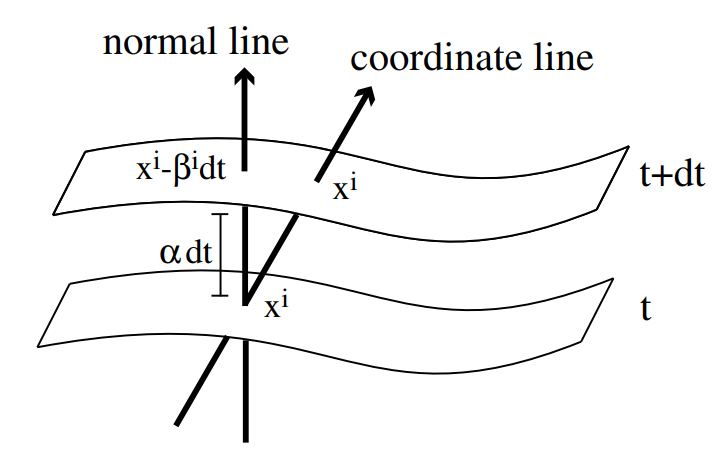
\includegraphics[width=0.5\textwidth]{Figures/Definitions_of_the_3+1_quantities.png}
\caption{Geometric definition of the lapse function $\alpha$ and the shift vector $\beta^i$. The lapse function $\alpha$ is the proper time between two adjacent hypersurfaces $\Sigma_t$ and $\Sigma_{t+dt}$ measured by \textit{Eulerian observers}. The shift vector $\beta^i$ is the relative velocity between the \textit{Eulerian observers} and the lines of constant spatial coordinates. \cite{Introduction_to_3+1_numerical_relativity}}
\end{figure}

In this work, we are interested in specifying initial conditions starting from a known spacetime metric $g_{ab}$~. Thus, we need to calculate the previously mentioned 3+1 quantities from $g_{ab}$~, which can be done by performing a 3+1 split of $g_{ab}$~. This split is done by writing $g_{ab}$~as a function of $\alpha$~, $\beta^i$~and $\gamma_{ij}$~:
%
\begin{align}
 ds^2 = (-\alpha^2 + \beta_i \beta^i) ~ dt^2 
     + 2 \beta_i ~ dt dx^i 
     + \gamma_{ij} ~ dx^i dx^j,
\end{align}
%
or, more explicitly,
%
\begin{align}
    \begin{aligned}
        g_{\mu\nu} = \begin{pmatrix} 
            -\alpha^2 + \beta_k \beta^k & \beta_i \\
            \beta_j & \gamma_{ij} 
        \end{pmatrix}, 
        & \quad \quad \quad 
        g^{\mu\nu} = \begin{pmatrix} 
            -1/\alpha^2 & \beta^i/\alpha^2 \\
            \beta^j/\alpha^2 & \gamma^{ij} - \beta^i \beta^j/\alpha^2
        \end{pmatrix}.
    \end{aligned}
\end{align}

Using this split, it becomes easy to obtain $\alpha$~, $\beta^i$~and $\gamma_{ij}$~from $g_{ab}$~, from which we can obtain the extrinsic curvature $K_{\mu\nu}$~using the fact that
%
\begin{align}
 K_{ij} = \frac{D_i \beta_j + D_j \beta_i - \partial_t \gamma_{ij}}{2 \alpha},
\end{align}
%
where $D_\mu := (\delta^\alpha_\mu + n^\alpha n_\mu) \nabla_\alpha$~is the projection of the covariant derivative onto the hypersurface and $n$~is the normal vector to the hypersurface, with components given by
%
\begin{align}
    \begin{aligned}
        n^\mu = (1/\alpha,~-\beta^i/\alpha), 
        & \quad \quad \quad n_\mu = (-\alpha,~0).
    \end{aligned}
\end{align}

We can also obtain the acceleration of the \textit{Eulerian observers} $a^i$~as
\begin{align}
 a^i = \gamma^{ij} \partial_j(\ln \alpha).
\end{align}


%%%%%%%%%%%%%%%%%%%%%%%%%%%%%%%%%%%%%%%%%%%%%%%%%%%%%%%%%%%%%%%%%%%%%%%%
\section{Hyperboloidal Compactification}
\label{section:compactification}

In this work, we are interested in studying how waves behave at future null infinity, making it useful to compactify our spacetime in such a way that allows us to study the asymptotic behavior of our solutions numerically. To accomplish this, we will employ a specific set of coordinates called \textit{hyperboloidal coordinates} \cite{Hyperboloidal_layers_for_hyperbolic_equations_on_unbounded_domains,The_evolution_of_hyperboloidal_data_with_the_dual_foliation_formalism_Mathematical_analysis_and_wave_equation_tests}. 

The hyperboloidal coordinates $(t, r)$ are related to the usual spherical coordinates $(T, R)$ by the \textit{height function} $H(R)$~and the \textit{compress function} $\Omega(r)$~as follows:
%
\begin{align}
 T = t + H(R), 
     \quad \quad \quad R = \Omega^{-1}(r) \, r.
\end{align}
%
The angular coordinates remain unchanged. This transformation gives rise to the Jacobian matrix
%
\begin{align}
    \left(J^{Hyp}\right)_{\alpha'}^{\ \ \beta} = 
    \begin{pmatrix}
        1 & -H'(r) & 0 & 0 \\
        0 & \frac{L(r)}{\Omega^2(r)} & 0 & 0 \\
        0 & 0 & 1 & 0 \\
        0 & 0 & 0 & 1
    \end{pmatrix} \; ,
\end{align}
%
where $H'(r)$ denotes the derivative of the height function with respect to $R$ written as a function of $r$, and $L(r)$ is defined as
%
\begin{align}
 L(r) \equiv \Omega(r) - r \, \partial_r \Omega(r) \; .
\end{align}

It is important to note that, even though there is freedom to choose the height and the compress function, we must require that, asymptotically in $R$, or equivalently, as $\Omega$ approaches zero, we have
%
\begin{align}
    1 - H' \sim O(\Omega^2) \, .
\end{align}

Since the solutions to our equations decay as we approach null infinity, it is useful to rescale our spacetime in such a way that our solutions are of order one through space. Given a spacetime with metric $g_{ab}$~, we can rescale it by a strictly positive, smooth scalar function $\Omega$~to obtain a new metric $\tilde{g}_{ab}$~:
%
\begin{align}
    \tilde{g}_{ab} = \Omega^2 g_{ab},
\end{align}
%
This rescaling is called a \textit{conformal transformation} and the function $\Omega$~ is called the \textit{conformal factor}. If $g_{ab}$~is a Lorentzian metric, then a vector $v^a$~is timelike, null or spacelike with respect to $g_{ab}$~ if and only if it is timelike, null or spacelike with respect to $\tilde{g}_{ab}$~, meaning that the causal structure of the spacetime is preserved under conformal compactification \cite{wald:1984}. 

After applying both the coordinate transformation to hyperboloidal coordinates and the conformal transformation, we obtain a new metric $\tilde{g}_{ab}$~, which on Cartesian coordinates is given by

\begin{align}
    \tilde{g}_{ab} = 
    \begin{pmatrix}
        -\Omega^2(r) & -\frac{x H(r) L(r)}{r} & -\frac{y H(r) L(r)}{r} & -\frac{z H(r) L(r)}{r} \\
        -\frac{x H(r) L(r)}{r} & \frac{(y^2 + z^2) \mathcal{R}^2(r) + r^2 x^2 L^2(r) \Xi(r)}{r^4} & \frac{x y (-\mathcal{R}^2(r) + r^2 L^2(r) \Xi(r))}{r^4} & \frac{x z (-\mathcal{R}^2(r) + r^2 L^2(r) \Xi(r))}{r^4} \\
        -\frac{y H(r) L(r)}{r} & \frac{x y (-\mathcal{R}^2(r) + r^2 L^2(r) \Xi(r))}{r^4} & \frac{(x^2 + z^2) \mathcal{R}^2(r) + r^2 y^2 L^2(r) \Xi(r)}{r^4} & \frac{y z (-\mathcal{R}^2(r) + r^2 L^2(r) \Xi(r))}{r^4} \\
        -\frac{z H(r) L(r)}{r} & \frac{x z (-\mathcal{R}^2(r) + r^2 L^2(r) \Xi(r))}{r^4} & \frac{y z (-\mathcal{R}^2(r) + r^2 L^2(r) \Xi(r))}{r^4} & \frac{(x^2 + y^2) \mathcal{R}^2(r) + r^2 z^2 L^2(r) \Xi(r)}{r^4}
    \end{pmatrix} \; ,
\end{align}
%
where we have defined $\Xi(r)$ and $\mathcal{R}(r)$ as
%
\begin{align}
    \Xi(r) = \frac{1 - H^2(r)}{\Omega^2(r)} \; , \quad \quad \quad \mathcal{R}(r) = r - R_i + R_i \Omega(r) \; ,
\end{align}
%
with $R_i$ being the interface radius, which we will now briefly discuss.

In some applications, it may be useful to consider a flat slice where most of the dynamics happen, followed by a hyperboloidal slice, which allows us to study the decay of our solution as it approaches future null infinity \cite{Hyperboloidal_layers_for_hyperbolic_equations_on_unbounded_domains,The_evolution_of_hyperboloidal_data_with_the_dual_foliation_formalism_Mathematical_analysis_and_wave_equation_tests}. That scenario can be achieved using \textit{hyperboloidal layers}, which consist of performing a transition from flat slices to hyperboloidal slices at a chosen interface radius $R_i$, making it such that we achieve a hyperboloidal slice after some transition length $l_t$. The details of this transition will be further discussed in section \ref{section:hyp_layers_wave}.


%%%%%%%%%%%%%%%%%%%%%%%%%%%%%%%%%%%%%%%%%%%%%%%%%%%%%%%%%%%%%%%%%%%%%%%%
\section{The Wave Equation}
\label{section:wave_equation}

The wave equation is a symmetric hyperbolic partial differential equation that describes the propagation of all types of wave-like phenomena. In the study of gravitational waves, this equation is of particular importance due to its structural similarity to the Einstein field equations on the \textit{Generalized Harmonic Gauge (GHG)}. The wave equation, in its simpler form, is given by
%
\begin{align}
    \Box_g \Psi = S,
    \label{eq:wave_equation_simple}
\end{align}
%
where $\Box_g$ is the d'Alembert operator, $\Psi$ is the scalar field, and $S$ is a source term. The Einstein equations in the GHG can be written as
%
\begin{align}
    \Box_g g_{ab} = 2 g^{cd} g^{ef} (\partial_e g_{ca} \partial_f g_{db} - \Gamma_{ace} \Gamma_{bdf}),
\end{align}
%
where $g_{ab}$ is the spacetime metric, $\Gamma_{abc}$ are the Christoffel symbols, and $g^{ab}$ are the inverse metric \cite{A_new_generalized_harmonic_evolution_system}. The similarity between these two equations allows us to study the wave equation as a model for gravitational waves.

It is important to note that when we perform a conformal transformation of the spacetime like the one described in section \ref{section:compactification}, the d'Alembert operator in the new metric $\tilde{g}_{ab}$~becomes
%
\begin{align}
    \Box_{\tilde{g}} \tilde{\psi} = \tilde{g}^{ab} \tilde{\nabla}_a \tilde{\nabla}_b \tilde{\psi}
    &= \Omega^{s-2} g^{ab} \nabla_a \nabla_b \psi + s \Omega^{s-3} \psi\, g^{ab} \nabla_a \nabla_b \Omega \\
    &\quad + s(n + s - 3) \Omega^{s-4} \psi\, g^{ab} \nabla_a \Omega \nabla_b \Omega
    \label{eq:conformal_wave_equation1}
\end{align}
%
where $s$~is the conformal weight of the scalar field $\psi$ (which we can choose freely)~and $n$~is the dimension of the spacetime \cite{wald:1984}. In this work, we will be working in a four-dimensional spacetime, so $n = 4$~. The conformal weight $s$~will be chosen to be $s = -1$ to simplify the expression of equation \eqref{eq:conformal_wave_equation1}. Thus, we have
%
\begin{align}
    \tilde{g}^{ab} \tilde{\nabla}_a \tilde{\nabla}_b \tilde{\psi} 
 =&~\Omega^{-3} g^{ab} \nabla_a \nabla_b \psi 
 - \Omega^{-4} \psi\, g^{ab} \nabla_a \nabla_b \Omega,
    \label{eq:conformal_wave_equation2}
\end{align}
%
We can now substitute \eqref{eq:wave_equation_simple} into \eqref{eq:conformal_wave_equation2} and write the resulting equation in terms of the rescaled quantities, obtaining
%
\begin{align}
    \tilde{g}^{ab} \tilde{\nabla}_a \tilde{\nabla}_b \tilde{\psi} 
 =&~\Omega^{-3} S 
 - \Omega^{-1} \tilde{\psi} \bigg( 
    \tilde{g}^{ab} \tilde{\nabla}_a \tilde{\nabla}_b \Omega 
 - 2 \Omega^{-1} \tilde{g}^{ab} \tilde{\nabla}_a \Omega \tilde{\nabla}_b \Omega \bigg),
\end{align}
%
which is the wave equation for the rescaled scalar field $\tilde{\psi}$~in the compactified spacetime with metric $\tilde{g}_{ab}$~.

To solve the previous equation numerically, it is useful to do a 3+1 decomposition of spacetime and write the system as a set of first-order partial differential equations. To do that, we start by employing the 3+1 split of the metric $\tilde{g}_{ab}$~described in section \ref{section:3+1_formalism} and define the time reduction variable $\tilde{\Pi}$~and the spatial reduction variables $\tilde{\phi}_i$~as
%
\begin{align}
    \Pi = - \mathcal{L}_n \tilde{\psi} \;  \quad \quad \quad \phi_i = \tilde{D}_i \tilde{\psi} \; ,
\end{align}
%
where $\mathcal{L}_n$~is the Lie derivative along the normal vector to the hypersurface $n^a$~, and $\tilde{D}_i$~is the projection of the covariant derivative onto the hypersurface. It is important to note that these definitions introduce new constraints to our system, given by
%
\begin{align}
    \begin{cases}
        \mathcal{L}_n \tilde{\psi} + \Pi \overset{!}{=} 0 \\
        \tilde{D}_i \tilde{\psi} - \phi_i \overset{!}{=} 0
    \end{cases}\,,
\end{align}
%
where $\overset{!}{=}$ denotes that we may allow for small violations of these constraints due to numerical errors. The second constraint is of particular importance as we will see later in section \ref{section:hyp_wave}. Due to this importance, we will denote it as $C_i$.

Using the previous definitions, we can write the wave equation as a set of first-order partial differential equations as
%
\begin{align}
    \begin{cases}
        \partial_t \tilde{\psi} = - \tilde{\alpha} \tilde{\Pi} + \beta^i \tilde{\phi}_i \\
        \partial_t \tilde{\phi}_i = - \tilde{\alpha} (\tilde{D}_i \tilde{\Pi}) - (\tilde{D}_i \tilde{\alpha}) \tilde{\Pi} + \beta^j \partial_j \tilde{\phi}_i + \tilde{\phi}_j \partial_i \beta^j \\
        \partial_t \tilde{\Pi} = - \tilde{\alpha} \tilde{a}^i \tilde{\phi}_i - \tilde{\alpha} \tilde{\gamma}^{ij} \tilde{D}_j \tilde{\phi}_i + \tilde{\alpha} \tilde{K} \tilde{\Pi} + \beta^i \tilde{D}_i \tilde{\Pi} \\
        \hspace{3.5em} - \tilde{\alpha} \Omega^{-1} \Big( \tilde{g}^{ab} \tilde{\nabla}_a \tilde{\nabla}_b \Omega - 2 \Omega^{-1} \tilde{g}^{ab} \tilde{\nabla}_a \Omega \tilde{\nabla}_b \Omega \Big) \tilde{\psi} + \tilde{\alpha} \Omega^{-3} S
    \end{cases}\,.
    \label{eq:wave_equation_3+1}
\end{align}

It is also necessary to calculate the characteristic variables of our system and their respective speeds. To do so, we start by calculating the principal symbol of our system and its eigenvalues, obtaining advection equations for the characteristic variables
%
\begin{align}
    \begin{cases}
        \partial_t \tilde{\psi} = 0 \\
        \partial_t (\tilde{\Pi} \pm \tilde{\phi}_s) = - (-\beta^s \pm \tilde{\alpha}) \partial_s (\tilde{\Pi} \pm \tilde{\phi}_s)
    \end{cases}\,,
\end{align}
%
where $\tilde{\phi}_s = \tilde{\phi}_i s^i$~(it is important to note that this definition does not let~$\tilde{\phi}_i$~and~$s^i$~commute) and similarly for $\beta^s$, with $s^i$~being an arbitrary unit spatial vector. From this, we can identify the characteristic variables as 
%
\begin{align}
    \begin{cases}
        u_0 = \tilde{\psi} \\
        u_\pm = \tilde{\Pi} \pm \tilde{\phi}_s \\
        (u_2)_i = (\delta_i^j - s_i s^j) \tilde{\phi}_j
    \end{cases}\,,
\end{align}
%
with the associated characteristic speeds being
%
\begin{align}
    \begin{cases}
        v_0 = 0 \\
        v_\pm = -\beta^s \pm \tilde{\alpha} \\
        v_2 = -\beta^s
    \end{cases}\,.
\end{align}

In order to keep constraint violations from growing exponentially, it may be useful to add multiples of the constraint $C_i$~to the evolution equations of our system since doing so does not alter the physical behavior of the system, but it improves numerical stability. Doing so, we obtain the final form of our system as
%
\begin{align}
    \begin{cases}
        \partial_t \tilde{\psi} = - \tilde{\alpha} \tilde{\Pi} + \beta^i \tilde{\phi}_i + (1 + \gamma_1) \beta^i (\tilde{D}_i \tilde{\psi} - \tilde{\phi}_i) \\
        \partial_t \tilde{\phi}_i = - \tilde{\alpha} (\tilde{D}_i \tilde{\Pi}) - (\tilde{D}_i \tilde{\alpha}) \tilde{\Pi} + \beta^j \partial_j \tilde{\phi}_i + \tilde{\phi}_j \partial_i \beta^j + \gamma_2 \tilde{\alpha} (\tilde{D}_i \tilde{\psi} - \tilde{\phi}_i) \\
        \partial_t \tilde{\Pi} = - \tilde{\alpha} \tilde{a}^i \tilde{\phi}_i - \tilde{\alpha} \tilde{\gamma}^{ij} \tilde{D}_j \tilde{\phi}_i + \tilde{\alpha} \tilde{K} \tilde{\Pi} + \beta^i \tilde{D}_i \tilde{\Pi} \\
        \hspace{3.5em} - \tilde{\alpha} \Omega^{-1} \Big( \tilde{g}^{ab} \tilde{\nabla}_a \tilde{\nabla}_b \Omega - 2 \Omega^{-1} \tilde{g}^{ab} \tilde{\nabla}_a \Omega \tilde{\nabla}_b \Omega \Big) \tilde{\psi} + \tilde{\alpha} \Omega^{-3} S + \gamma_3 \beta^i (\tilde{D}_i \tilde{\psi} - \tilde{\phi}_i)
    \end{cases}\,,
    \label{eq:wave_equation_constraint_violation}
\end{align}
%
where $\gamma_1$~, $\gamma_2$~, and $\gamma_3$~are free parameters which quantify the constraint violation we allow in our system. This addition will also change the characteristic variables and their respective speeds. Choosing $\gamma_3 = \gamma_1 \gamma_2$~for convenience, we obtain the characteristic variables as
%
\begin{align}
    \begin{cases}
        u_0 = \tilde{\psi} \\
        u_\pm = \tilde{\Pi} \pm \tilde{\phi}_s - \gamma_2 \tilde{\psi} \\
        (u_2)_i = (\delta_i^j - s_i s^j) \tilde{\phi}_j
    \end{cases}\,,
\end{align}
%
with the respective characteristic speeds being
%
\begin{align}
    \begin{cases}
        v_0 = - (1 + \gamma_1) \beta^s \\
        v_\pm = -\beta^s \pm \tilde{\alpha} \\
        v_2 = -\beta^s
    \end{cases}\,.
\end{align}


%%%%%%%%%%%%%%%%%%%%%%%%%%%%%%%%%%%%%%%%%%%%%%%%%%%%%%%%%%%%%%%%%%%%%%%%
\section{The Cubic Wave Equation}
\label{section:cubic_wave_equation}
\cleardoublepage

%%%%%%%%%%%%%%%%%%%%%%%%%%%%%%%%%%%%%%%%%%%%%%%%%%%%%%%%%%%%%%%%%%%%%%%%
%                                                                      %
%     File: Thesis_Implementation.tex                                  %
%     Tex Master: Thesis.tex                                           %
%                                                                      %
%     Author: Andre C. Marta                                           %
%     Last modified :  4 Mar 2024                                      %
%                                                                      %
%%%%%%%%%%%%%%%%%%%%%%%%%%%%%%%%%%%%%%%%%%%%%%%%%%%%%%%%%%%%%%%%%%%%%%%%

\chapter{Numerical Setup}
\label{chapter:numerical_setup}

In this chapter, we will describe the numerical setup of the \texttt{bamps} code. We will start by discussing the grid setup in section \ref{section:grid}, followed by the numerical method used to solve the partial differential equation systems in section \ref{section:Numerical_Method} and a brief description of how \texttt{bamps} handles patch boundaries in section \ref{section:Patch_Boundaries}. Finally, we will discuss the Adaptive Mesh Refinement (AMR) strategy employed by \texttt{bamps} in section \ref{section:amr}.

%%%%%%%%%%%%%%%%%%%%%%%%%%%%%%%%%%%%%%%%%%%%%%%%%%%%%%%%%%%%%%%%%%%%%%%%
\section{Grid Setup}
\label{section:grid}

The \texttt{bamps} code uses a multi-patch grid setup to cover the computational domain. Even though \texttt{bamps} is capable of supporting both a cubed-ball grid and a cubed-sphere grid, in this work we will only use the cubed-ball grid. The grid is composed of several patches which are shaped like deformed cubes that fit together to cover the domain. Each patch is mapped by two different coordinate systems: the local patch coordinates $(\bar{x},\bar{y},\bar{z})$ and the global Cartesian coordinates $(x,y,z)$.

The cubed-ball grid consists of a central cube surrounded by six deformed cube patches that form a spherical shell around the central cube forming a transition shell, which is itself surrounded by six more deformed cube patches that form the outer spherical shell. In the central cube, the local patch coordinates and the global Cartesian coordinates are identical, i.e., $(\bar{x},\bar{y},\bar{z}) = (x,y,z)$. However, in the other patches, a coordinate transformation must be applied to map the local patch coordinates to the global Cartesian coordinates. This transformation is performed in two steps: first, the local coordinates are transformed to temporary global coordinates $(\tilde{x},\tilde{y},\tilde{z})$, which are then transformed to the final global Cartesian coordinates $(x,y,z)$ by performing a rotation of the patch to their correct placement on the sphere. The transformation from local patch coordinates to temporary global coordinates is given by
%
\begin{align}
    x_t = \frac{\bar{x}}{\bar{s}} \; , \quad \quad y_t = \frac{\bar{x}}{\bar{s}} \bar{y} \; ,  \quad \quad z_t = \frac{\bar{x}}{\bar{s}} \bar{z} \; ,
\end{align}
%
where, for the outer patches,
%
\begin{align}
    \bar{s} = \sqrt{1 + \bar{y}^2 + \bar{z}^2} \; 
\end{align}
%
and for the inner patches,
%
\begin{align}
    \bar{s}(\lambda) = \sqrt{\frac{1 + 2\lambda}{1 + \lambda (\bar{y}^2 + \bar{z}^2)}} \; , \quad \quad \quad \lambda = \frac{\bar{x}^2 - \bar{x}_0^2}{\bar{x}_1^2 - \bar{x}_0^2} ,
\end{align}
%
where $\bar{x}_0$ and $\bar{x}_1$ are the boundaries of the patch in the local coordinates \cite{Pseudospectral_method_for_gravitational_wave_collapse}.

Each patch can be further divided into several subpatches, which are smaller cubes that allow for a more refined grid in specific regions of the domain. When dividing a patch into subpatches, the division is done such that subgrids of two neighboring patches match, and that neighboring patches and subpatches have the same grid-point positions on their respective boundaries. In figure \ref{fig:cubed_ball_grid}, we show an example of a cubed-ball grid divided into subpatches.

\begin{figure}[t!]
    \centering
    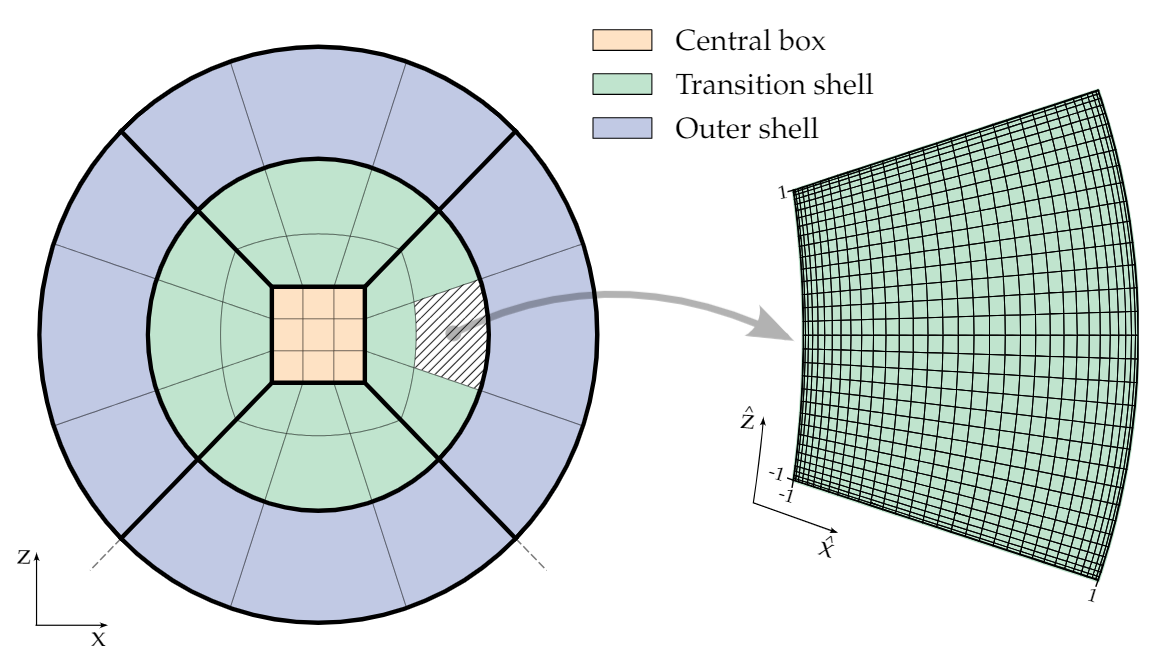
\includegraphics[width=0.75\textwidth]{Figures/Cubed_Ball.png}
    \caption{Two-dimensional sketch of the \texttt{bamps} cubed-ball grid layout. The grid is composed of several patches shaped like deformed cubes. These patches can be further divided into subpatches. Each subpatch is covered by Gauss-Lobatto grids. \cite{Pseudospectral_method_for_gravitational_wave_collapse}}
    \label{fig:cubed_ball_grid}
\end{figure}

%%%%%%%%%%%%%%%%%%%%%%%%%%%%%%%%%%%%%%%%%%%%%%%%%%%%%%%%%%%%%%%%%%%%%%%%
\section{Numerical Method}
\label{section:Numerical_Method}

\texttt{bamps} uses the method of lines to solve the system of partial differential equations, meaning that it treats time as a continuous variable and space as discrete. To integrate fields forward in time, a fourth-order Runge-Kutta scheme is employed. The spatial discretization is performed using Gauss-Lobatto collocation points, which is done by mapping the local patch coordinates $(\bar{x},\bar{y},\bar{z})$ to the reference cube coordinates $(\tilde{x},\tilde{y},\tilde{z}) \in [-1,1]^3$ and then using the Gauss-Lobatto points in each direction. The Gauss-Lobatto points in the $\tilde{x}$ direction are given by
%
\begin{align}
    \tilde{x}_\alpha = - \cos\left(\frac{\pi \alpha}{N_x -1}\right) \; ,
\end{align}
%
with $\alpha = 0,1,\ldots,N_x -1$ and $N_x$ being the number of grid points in the $\tilde{x}$ direction. The collocation points in the other two directions are defined similarly. It is important to note that the number of angular grid points must be the same in all patches to ensure that the grid points on the boundaries of neighboring patches match \cite{Pseudospectral_method_for_gravitational_wave_collapse}. A grid generated using Gauss-Lobatto points can be seen in figure \ref{fig:cubed_ball_grid}.

On each of the collocation points, all the evolution fields $u$ are expanded in each dimension in terms of Chebyshev polynomials $T_n(\tilde{x})$ as
%
\begin{align}
 u_{\alpha \beta \delta} = u(\tilde{x}_\alpha, \tilde{y}_\beta, \tilde{z}_\delta) = \sum_{l=0}^{N_z -1} c^x_n(\tilde{y}_\beta, \tilde{z}_\delta) \, T_n(\tilde{x}_\alpha) \; ,
\end{align}
%
and similarly for the $\tilde{y}$ and $\tilde{z}$ directions. This expansion enables a spectral representation of the fields, which is advantageous as it facilitates the analytical differentiation of our expansion through the analytical derivatives of the Chebyshev polynomials. Additionally, since for many applications the contribution of higher order polynomials decays exponentially, the numerical error in spectral methods usually decays exponentially with the resolution \cite{Numerical_Relativity_Solving_Einsteins_Equations_on_the_Computer}. \texttt{bamps} uses the pseudospectral approach, meaning that instead of storing the coefficients $c^x_n(\tilde{y}_\beta, \tilde{z}_\delta)$, it stores the values of the fields at the collocation points. The spatial derivatives of the fields are computed using matrix multiplication. For example, the derivative in the $\tilde{x}$ direction is computed as
%
\begin{align}
    (\partial_{\tilde{x}} u)_{\alpha \beta \delta} = \sum_{n=0}^{N_x -1} D_{\alpha n} u_{n \beta \delta} \; ,
\end{align}
%
where $D_{\alpha n}$ is the Gauss-Lobatto differentiation matrix
%
\begin{align}
    D_{\alpha\beta}=
    \begin{cases}
        -\frac{2(N_x-1)^2+1}{6} & \alpha=\beta=0 \\
        \frac{q_\alpha}{q_\beta}\frac{(-1)^{\alpha+\beta}}{\tilde{x}_\alpha-\tilde{x}_\beta} & \alpha\neq\beta \\
        \frac{-\tilde{x}_\beta}{2(1-\tilde{x}_\beta^2)} & \alpha=\beta=1,\cdots,N_x-2 \\
        \frac{2(N_x-1)^2+1}{6} & \alpha=\beta=N_x-1
    \end{cases} \, ,
\end{align}
%
where $q_\alpha = 2$ on the boundaries and $q_\alpha = 1$ otherwise \cite{Pseudospectral_method_for_gravitational_wave_collapse,Numerical_Relativity_Solving_Einsteins_Equations_on_the_Computer}.

To ensure numerical stability, \texttt{bamps} uses a filtering method to remove high-frequency modes. The filtering is applied after each full time step and consists of multiplying the fields by a filter matrix in each direction
%
\begin{align}
 (\mathcal{F}u)_{\alpha \beta \delta} = \sum_{n=0}^{N_x -1} \mathcal{F}_{n \alpha} u_{n \beta \delta} \; ,
\end{align}
%
where the filter matrix $\mathcal{F}_{n \alpha}$ is given by
%
\begin{align}
    \mathcal{F}_{\alpha \beta} = \sum_n S_{\alpha n} e^{-36 (n/(N_x - 1))^{64}} A_{n \beta} \; ,
\end{align}
%
where $S_{\alpha \beta}$ is the Chebyshev synthesis matrix and $A_{n \beta}$ is Chebyshev analysis matrix \cite{Pseudospectral_method_for_gravitational_wave_collapse,Numerical_Relativity_Solving_Einsteins_Equations_on_the_Computer}.

The \texttt{bamps} code also supports both 1-dimensional and 2-dimensional reductions, called the cartoon method. It is also able to handle mirror symmetries along the $x$, $y$, and $z$ directions \cite{The_evolution_of_hyperboloidal_data_with_the_dual_foliation_formalism_Mathematical_analysis_and_wave_equation_tests}.

%%%%%%%%%%%%%%%%%%%%%%%%%%%%%%%%%%%%%%%%%%%%%%%%%%%%%%%%%%%%%%%%%%%%%%%%
\section{Patching Boundary Conditions}
\label{section:Patch_Boundaries}

Since $\texttt{bamps}$ separates our domain into different patches, we need to impose boundary conditions between adjacent patches so that they can communicate data to each other. An effective way to impose these boundary conditions is to add appropriate penalty terms to the equations on these boundaries. This method, which we call \textit{Penalty Method}, imposes the needed boundary conditions while keeping the evolution equations at the boundary almost unchanged \cite{Pseudospectral_method_for_gravitational_wave_collapse,Spectral_methods_for_the_wave_equation_in_second-order_form}.

It consists of adding to the equation of motion of the incoming characteristic variable a term of the form $(u_-^{BC}  - u_-)$, where $u_-$ is the incoming \textit{characteristic variable}. Thus, if the boundary condition $u_-^{BC} = u_-$ is satisfied, the penalty terms vanish. We can then determine the appropriate penalty terms to add to the equation when written in their fundamental form by rewriting our evolution equations on the boundaries as functions of the characteristic variables, incorporating the penalty terms, and then transforming our system back \cite{Pseudospectral_method_for_gravitational_wave_collapse,Spectral_methods_for_the_wave_equation_in_second-order_form}. That way, the evolution equations \eqref{eq:wave_equation_3+1} on the boundary will get modified to
%
\begin{align}
    \left\{\begin{array}{@{}l@{}} 
        (\partial_t\tilde{\psi})^{BC} = \partial_t\tilde{\psi} \\
        (\partial_t\tilde{\Pi})^{BC} = \partial_t\tilde{\Pi} + \frac{1}{2} p \, \left( v_+(u_+^{BC}  - u_+) + v_- (u_-^{BC}  - u_-) \right) \\
        (\partial_t\tilde{\phi}_i)^{BC} = \partial_t\tilde{\phi}_i + \frac{1}{2} p \, n_i \, \left( v_+(u_+^{BC}  - u_+) - v_- (u_-^{BC}  - u_-) \right)  + p \, v_2 \left((u_2^{BC})_i  - (u_2)_i \right) \\
    \end{array}\right. ,
    \label{eq:penalty_terms}
\end{align}
%
where $p$ is the penalty coefficient, which can be determined from a semi-discrete energy analysis, and $n^i$ is the unit outgoing normal vector to the boundary. Even though in equation \eqref{eq:penalty_terms} the terms regarding every characteristic variable are included, it is important to note that only incoming characteristic variables are taken into account in this method; thus, if any of the characteristic speeds are greater than $0$, the penalty term associated will be null. 

If we allow for constraint violations in our system (as we did in equation \eqref{eq:wave_equation_constraint_violation}), the characteristic variables and their respective speeds will change, and we will need to modify the penalty terms accordingly, obtaining
%
\begin{align}
    \left\{\begin{array}{@{}l@{}} 
        (\partial_t\tilde{\psi})^{BC} = \partial_t\tilde{\psi} - p \, v_0 (u_0^{BC}  - u_0)\\
        (\partial_t\tilde{\Pi})^{BC} = \partial_t\tilde{\Pi} + \frac{1}{2} p \, \left( v_+(u_+^{BC}  - u_+) + v_- (u_-^{BC}  - u_-) \right) - 2 \, \gamma_2 \, p \, v_0 (u_0^{BC}  - u_0)\\
        (\partial_t\tilde{\phi}_i)^{BC} = \partial_t\tilde{\phi}_i + \frac{1}{2} p \, n_i \, \left( v_+(u_+^{BC}  - u_+) - v_- (u_-^{BC}  - u_-) \right)  + p \, v_2 \left((u_2^{BC})_i  - (u_2)_i \right) \\
    \end{array}\right. .
\end{align}

%%%%%%%%%%%%%%%%%%%%%%%%%%%%%%%%%%%%%%%%%%%%%%%%%%%%%%%%%%%%%%%%%%%%%%%%
\section{Adaptive Mesh Refinement}
\label{section:amr}

\texttt{bamps} has the capability of generating new grids during the evolution to supply additional resolution where needed to adequately represent the solution, and consolidate these fine grids back into fewer coarser ones once the improved resolution is no longer required (h-refinement). The code is also capable of adjusting the resolution in any individual grid (p-refinement). This process is called Adaptive Mesh Refinement (AMR).

The AMR procedure in \texttt{bamps} consists in:
%
\begin{enumerate}
    \item Evaluate the h-refinement indicator on each subpatch;
    \item Generate a set of initial h-refinement flags;
    \item Modify the h-refinement flags to satisfy the constraints for a 'legal' \texttt{bamps} grid;
    \item Apply the h-refinement operations;
    \item Perform load balancing to consolidate grids that are marked to be coarsened together;
    \item Apply h-coarsening operations;
    \item Evaluate the p-refinement indicator function on each grid;
    \item Apply p-refinement and p-coarsening operations;
    \item Apply final load balancing.
\end{enumerate}

It is possible to define several indicators to determine where refinement is needed. In this work, we will use the \textit{truncation error indicator}, which estimates the truncation error of our spectral expansion. This indicator is calculated by performing the spectral decomposition of the evolution fields as described in section \ref{section:Numerical_Method} and then constructing the sequence
%
\begin{align}
    \tilde{c}_i = \sqrt{\frac{1}{N} \sum_{k=1}^N c_i^k} \; , \quad \quad i = 1, 2, \ldots, \tilde{n} \;
\end{align}
%
where $\tilde{n}$ is the highest mode which is not affected by the filter described in section \ref{section:Numerical_Method}, and $k$ enumerates all $N$ lines of grid points. Then, an exponential is fitted to the sequence $\tilde{c}_i$ obtaining the indicator function
%
\begin{align}
    \epsilon = 10^{a \tilde{n} + b} \; ,
\end{align}
%
where $a$ and $b$ are the slope and the offset obtained from the least squares fit on the logarithm of the sequence $\tilde{c}_i$ \cite{Adaptive_hp_refinement_for_spectral_elements_in_numerical_relativity}.

It is important to note that the flags generated in the AMR procedure are then modified to ensure that the end state satisfies the constraints for a 'legal' \texttt{bamps} grid, as previously mentioned. This modification can be visualized in figure \ref{fig:amr_legal}. In a 'legal' \texttt{bamps} grid, each subpatch is not allowed to be more than one refinement level apart from any of its neighbors, and the grid structure must satisfy a 1:2 condition. This means that if a subpatch is refined, all its neighbors must either be at the same refinement level or one level coarser. This is done to ensure that the grid structure remains consistent and that the numerical methods used in \texttt{bamps} can operate correctly across patch boundaries \cite{Adaptive_hp_refinement_for_spectral_elements_in_numerical_relativity}.

\begin{figure}[t!]
    \centering
    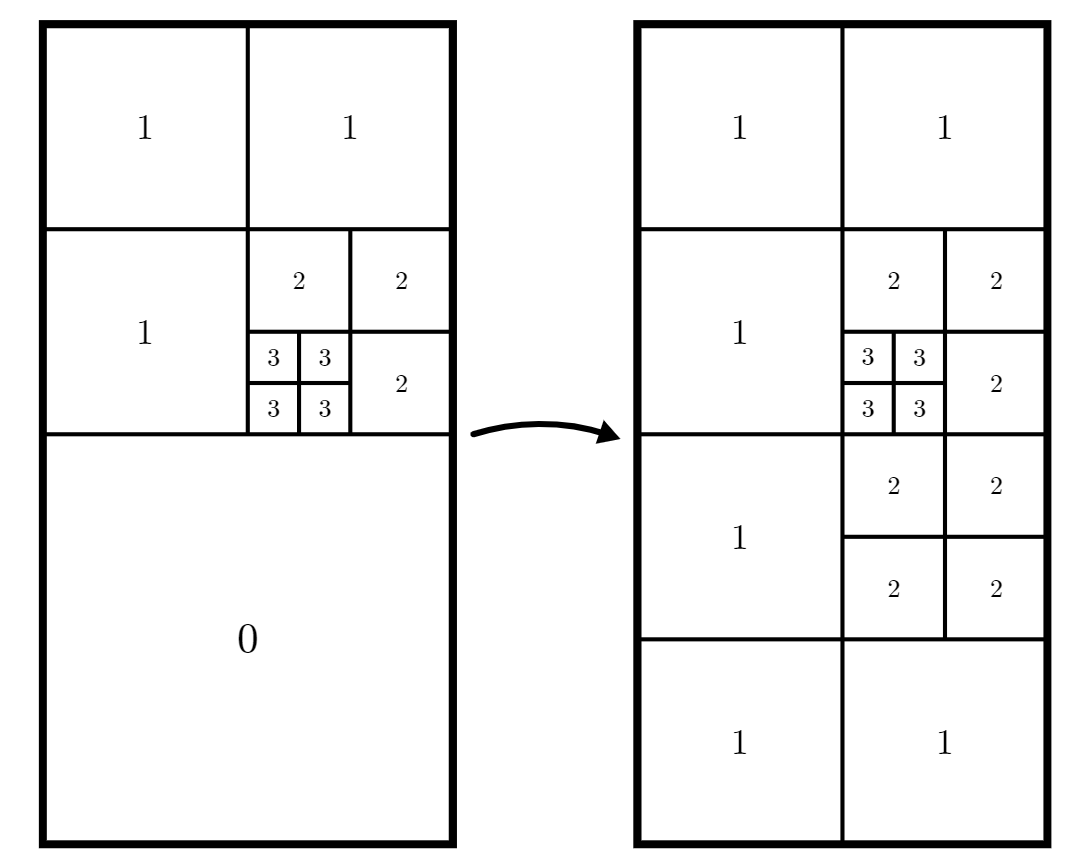
\includegraphics[width=0.5\textwidth]{Figures/AMR.png}
    \caption{Example of a grid that does not satisfy the constraints for a 'legal' \texttt{bamps} grid (left) and the same grid after the modification of the h-refinement flags to obey these constraints (right). In a 'legal' \texttt{bamps} grid, each subpatch is not allowed to be more than one refinement level apart from any of its neighbors, and the grid structure must satisfy a 1:2 condition. Thus, if a subpatch is refined, all its neighbors must either be at the same refinement level or one level coarser. This change in refinement level is made to ensure that the grid structure remains consistent and that the numerical methods used in \texttt{bamps} can operate correctly across patch boundaries \cite{Adaptive_hp_refinement_for_spectral_elements_in_numerical_relativity}.}
    \label{fig:amr_legal}
\end{figure} % file "Thesis_Implementation.tex"
\cleardoublepage

%\input{Thesis_new_file} % add new .tex files for new chapters
%\cleardoublepage

%\input{Thesis_new_file} % add new .tex files for new chapters
%\cleardoublepage

%\input{Thesis_new_file} % add new .tex files for new chapters
%\cleardoublepage

%%%%%%%%%%%%%%%%%%%%%%%%%%%%%%%%%%%%%%%%%%%%%%%%%%%%%%%%%%%%%%%%%%%%%%%%
%                                                                      %
%     File: Thesis_Results.tex                                         %
%     Tex Master: Thesis.tex                                           %
%                                                                      %
%     Author: Andre C. Marta                                           %
%     Last modified :  4 Mar 2024                                      %
%                                                                      %
%%%%%%%%%%%%%%%%%%%%%%%%%%%%%%%%%%%%%%%%%%%%%%%%%%%%%%%%%%%%%%%%%%%%%%%%

\chapter{Results}
\label{chapter:results}

Insert your chapter material here.


%%%%%%%%%%%%%%%%%%%%%%%%%%%%%%%%%%%%%%%%%%%%%%%%%%%%%%%%%%%%%%%%%%%%%%%%
\section{Wave Equation in Hyperboloidal Slices}
\label{section:hyp_wave}

The first step towards our goal is to implement the wave equation from equation \eqref{eq:wave_equation_3+1} in hyperboloidal slices. We will construct our hyperboloidal slices using 
%
\begin{align}
    H(R) = \frac{2 R^2 + s^2 - \sqrt{4 R^2 s^2 + s^4}}{2 \sqrt{R^2 + 1}} \,, \quad \quad \quad \Omega(r) = 1 - \frac{r^2}{s^2} \,,
\end{align}
%
as heigh and compress functions respectively, where $s$ is a free parameter that controls where null infinity is located. The details of this construction were discussed in section \ref{section:compactification}. This particular choice of heigh and compress functions is of particular interest since it leads to a constant outgoing characteristic speed, which has the advantage of keeping the shape of the waves as they propagate \cite{Hyperboloidal_layers_for_hyperbolic_equations_on_unbounded_domains,The_evolution_of_hyperboloidal_data_with_the_dual_foliation_formalism_Mathematical_analysis_and_wave_equation_tests}. This, however comes with the disadvantage of having an incoming characteristic speed that goes to zero as we approach null infinity. This is an acceptable trade-off since we are not expecting incoming waves in our setup. In figure \ref{fig:hyp_speeds} we can see how the incoming and outgoing light speeds vary along our computational domain.

\textcolor{red}{INSERT FIGURE WITH SPEEDS HERE}

Giving the initial conditions 
%
\begin{align}
    sjdjfçlsdg
\end{align}
%
and setting $s = 30$, we obtain the evolution shown in figures \ref{fig:hyp_wave1} and \ref{fig:hyp_wave2}, which satisfies the 


%%%%%%%%%%%%%%%%%%%%%%%%%%%%%%%%%%%%%%%%%%%%%%%%%%%%%%%%%%%%%%%%%%%%%%%%
\section{Wave Equation in Hyperboloidal Layers}
\label{section:hyp_layers_wave}




%%%%%%%%%%%%%%%%%%%%%%%%%%%%%%%%%%%%%%%%%%%%%%%%%%%%%%%%%%%%%%%%%%%%%%%%
\section{Cubic Wave Equation}
\label{section:hyp_cubic_wave}



 % file "Thesis_Results.tex"
\cleardoublepage

%%%%%%%%%%%%%%%%%%%%%%%%%%%%%%%%%%%%%%%%%%%%%%%%%%%%%%%%%%%%%%%%%%%%%%%%
%                                                                      %
%     File: Thesis_Conclusions.tex                                     %
%     Tex Master: Thesis.tex                                           %
%                                                                      %
%     Author: Andre C. Marta                                           %
%     Last modified :  4 Mar 2024                                      %
%                                                                      %
%%%%%%%%%%%%%%%%%%%%%%%%%%%%%%%%%%%%%%%%%%%%%%%%%%%%%%%%%%%%%%%%%%%%%%%%

\chapter{Conclusions}
\label{chapter:conclusions}

Insert your chapter material here.


% ----------------------------------------------------------------------
\section{Achievements}
\label{section:achievements}

The major achievements of the present work.


% ----------------------------------------------------------------------
\section{Future Work}
\label{section:future}

A few ideas for future work.

 % file "Thesis_Conclusions.tex"
\cleardoublepage

% ----------------------------------------------------------------------
%  Bibliography
% ----------------------------------------------------------------------

% Add entry in the table of contents as chapter
\phantomsection
\addcontentsline{toc}{chapter}{\bibname}

% Include all references in .bib file, even non-cited ones...
%\nocite{*} % this should be used carefully because it is not correct!

% Produces the bibliography section when processed by BibTeX
%
% Bibliography style
% > entries ordered alphabetically
%\bibliographystyle{plain}
% > unsorted with entries appearing in the order in which the citations appear.
%\bibliographystyle{unsrt}
% > entries ordered alphabetically, with first names and names of journals and months abbreviated
%\bibliographystyle{abbrv}
% > entries ordered alphabetically, with reference markers based on authors' initials and publication year
%\bibliographystyle{alpha}
%
% Replacement bibliography styles provided by 'natbib' package
% (plainnat.bst, abbrvnat.bst, unsrtnat.bst )
% > entries ordered alphabetically
%\bibliographystyle{plainnat}
% > unsorted with entries appearing in the order in which the citations appear.
%\bibliographystyle{unsrtnat}
% > entries ordered alphabetically, with first names and names of journals and months abbreviated
%\bibliographystyle{abbrvnat} % <<<<< SELECT IF USING REFERENCES BY AUTHOR/YEAR
% > entries ordered alphabetically, with reference markers based on authors' initials and publication year
%\bibliographystyle{alpha}
%
% Custom bibliography style adapted from 'natbib' package
%   (based on http://tex.stackexchange.com/questions/5053/is-it-possible-to-get-unsrt-abbrv-bibliography)
%   (unsrtnat.bst + abbrvnat.bst -> abbrvunsrtnat.bst)
%   (original files copied from:
%   http://tug.ctan.org/macros/latex/contrib/natbib/abbrvnat.bst
%   http://tug.ctan.org/macros/latex/contrib/natbib/unsrtnat.bst
% > unsorted with entries appearing in the order in which the citations appear, with first names and names of journals and months abbreviated.
\bibliographystyle{abbrvunsrtnat} % <<<<< SELECT IF USING REFERENCES BY NUMBER (CITATION ORDER)

% External bibliography database file in the BibTeX format
\bibliography{Thesis_Bibliography_DB} % file "Thesis_Bibliography_DB.bib"

\cleardoublepage

% ----------------------------------------------------------------------
%  Appendix (optional)
%
%  CAUTION: 1) the main document (up to the conclusions) shall not exceed 80 pages
%           2) the document shall not exceed a total of 100 pages (per IST regulations)
% ----------------------------------------------------------------------


% ----------------------------------------------------------------------
\end{document}
% ----------------------------------------------------------------------
